\documentclass[12pt,a4paper]{article}

% ==============================================================================
% PACKAGES: 100% PDFLATEX COMPATIBLE (NO FONTSPEC - STABLE COMPILATION)
% ==============================================================================
\usepackage[utf8]{inputenc}
\usepackage[T1]{fontenc}
\usepackage{lmodern}
\usepackage[margin=1.8cm,top=2.5cm,bottom=2.2cm,headheight=22pt]{geometry}
\usepackage{amsmath,amssymb}
\usepackage{booktabs}
\usepackage{graphicx}
\usepackage{hyperref}
\usepackage{fancyhdr}
\usepackage{cite}
\usepackage{tabularx}
\usepackage{chngcntr}
\usepackage{xcolor}

% Microtypography & spacing adjustments to eliminate overfull boxes
\emergencystretch=1.5em

% Unicode compatibility mappings for pdfLaTeX
\DeclareUnicodeCharacter{0110}{\DJ}
\DeclareUnicodeCharacter{0111}{\dj}
\DeclareUnicodeCharacter{2014}{---}
\DeclareUnicodeCharacter{1EA9}{\^{a}}
\DeclareUnicodeCharacter{1EA7}{\`{a}}

% Number equations, figures, and tables by section (e.g., Table 2.1, Figure 2.1)
\counterwithin{table}{section}
\counterwithin{figure}{section}
\counterwithin{equation}{section}

% Hyperlink configuration
\hypersetup{
    colorlinks=true,
    linkcolor=blue!80!black,
    citecolor=blue!70!black,
    urlcolor=blue!80!black,
    plainpages=false
}

% Header and Footer setup mirroring academic faculty template
\pagestyle{fancy}
\fancyhf{}
\setlength{\headheight}{22pt}
\fancyhead[L]{\fontsize{8.5}{10.5}\selectfont \textbf{HO CHI MINH CITY UNIVERSITY OF TECHNOLOGY (HCMUT)}\\
\textbf{FACULTY OF COMPUTER SCIENCE AND ENGINEERING}}
\fancyhead[R]{\fontsize{8.5}{10.5}\selectfont \textbf{CO3133 -- PROGRESS REPORT 3}\\
\textit{Academic Year 2026--2027}}
\renewcommand{\headrulewidth}{0.5pt}
\fancyfoot[L]{\fontsize{8.5}{10.5}\selectfont \textit{Enterprise Project HK261-DAGD1-558}}
\fancyfoot[R]{\fontsize{8.5}{10.5}\selectfont \textbf{Page \thepage}}
\renewcommand{\footrulewidth}{0.4pt}

\begin{document}

% ==============================================================================
% TITLE PAGE
% ==============================================================================
\begin{titlepage}
\hypersetup{pageanchor=false}
\centering
{\bfseries\large VIETNAM NATIONAL UNIVERSITY HO CHI MINH CITY\\[3pt]
HO CHI MINH CITY UNIVERSITY OF TECHNOLOGY\\[3pt]
FACULTY OF COMPUTER SCIENCE AND ENGINEERING\par}
\vspace{1.2cm}

% University / Department Emblem
\IfFileExists{HCMUT-logo.png}{
    
\includegraphics[width=3.2cm]{HCMUT-logo.png}
}{
    \framebox[3.2cm]{\rule{0pt}{3.2cm} \textbf{HCMUT -- CSE}}
}

\vspace{1.2cm}
{\Large\bfseries WEEKLY PROGRESS REPORT 3\par}
\vspace{0.25cm}
{\large Enterprise Semester (HK261) \quad\textbar\quad 12 Oct -- 25 Oct 2026\par}
\vspace{0.8cm}

\rule{\linewidth}{1.2pt}\\[0.4cm]
{\Large\bfseries Deep Learning-Based Durian Instance Segmentation and 3D Localization Using YOLOv8-Seg and Depth Sensing for Autonomous Agricultural Robots\par}
\vspace{0.2cm}
\rule{\linewidth}{1.2pt}

\vspace{0.6cm}
{\large\bfseries Course: Deep Learning and Its Applications (CO3133)\par}
\vspace{0.2cm}
{\normalsize Enterprise Project Code: \textbf{HK261-DAGD1-558}\par}
{\footnotesize (Autonomous Agricultural Spraying UGV with Dual-Axis Turret on Terraced Sloped Terrains)\par}

\vspace{1.2cm}
\begin{flushleft}
\large
\begin{tabular}{@{}ll@{}}
\textbf{Academic Supervisor:} & \textbf{MSc. Nguyen Quoc Minh} \\
                             & Department of Computer Science, HCMUT \\[0.3cm]
\textbf{Project Students:}    & \textbf{Tran Huu Hoang Long} \quad (Student ID: \textbf{2352704}) \\
                             & \textbf{Truong Gia Hy} \quad\quad\quad (Student ID: \textbf{2352458}) \\[0.3cm]
\textbf{Workstation Host:}   & Intel Core i5-13400F, RTX 3060 12\,GB, 32\,GB RAM \\
\textbf{Software Stack:}     & Windows 11 64-bit, PyTorch 2.3.0, Ultralytics 8.2 \\
\textbf{Embedded UGV Target:}& Raspberry Pi 5 (16\,GB), RealSense D453i, LiDAR C1M1 \\
\end{tabular}
\end{flushleft}

\vfill
{\large Ho Chi Minh City, October 2026\par}
\end{titlepage}
\hypersetup{pageanchor=true}

% ==============================================================================
% FRONT MATTER: CĐR MAPPING & CONTENTS
% ==============================================================================
\newpage
\pagenumbering{roman}

\section*{Course Learning Outcomes Compliance Summary}
\addcontentsline{toc}{section}{Course Learning Outcomes Compliance Summary}

This progress report satisfies the Course Learning Outcomes (Chu\^{a}n \dj\`{a}u ra --- C\DJ R / CLOs) of the \textbf{CO3133: Deep Learning and Its Applications} curriculum at Ho Chi Minh City University of Technology (HCMUT). Table~\ref{tab:cdr_front_mapping} provides an executive mapping between the specific project deliverables produced in this sprint and the official course learning rubrics.

\begin{table}[htbp]
\centering
\small
\caption{Executive mapping of sprint deliverables to CO3133 Course Learning Outcomes.}
\label{tab:cdr_front_mapping}
\begin{tabularx}{\textwidth}{l p{4.2cm} X c}
\toprule
\textbf{Course Outcome} & \textbf{Formal Rubric Definition} & \textbf{Direct Evidence in this Report} & \textbf{Status} \\
\midrule
\textbf{C\DJ R 8 (L.O.5.1)} & Empirically evaluate and compare deep learning models on domain datasets using standard metrics and error analysis. & 5-scenario ablation benchmark on NVIDIA RTX 3060 (Table~2.1), multi-task loss convergence curves (Figure~2.1), mosaic deactivation dynamics at Epoch 20, confusion matrix error decomposition, and Wilson 95\% confidence interval. & \textbf{Completed} \\
\addlinespace
\textbf{C\DJ R 9 (L.O.5.2)} & Analyze engineering trade-offs (accuracy, latency, compute, memory) to select optimal models for target deployments. & Rigorous trade-off analysis between YOLOv8n-seg and YOLOv8s-seg (Section~3.1), spatial resolution and batch size evaluation, Raspberry Pi 5 (16\,GB) resource allocation, and production gap review. & \textbf{Completed} \\
\addlinespace
\textbf{C\DJ R 4 (L.O.4.1)} & Implement and train computer vision models using modern deep learning frameworks on GPU workstations. & Full pipeline execution on NVIDIA RTX 3060 GPU using PyTorch 2.3.0 and Ultralytics 8.2, tracking training dynamics across 2,676 polygon-annotated images. & \textbf{Completed} \\
\addlinespace
\textbf{C\DJ R 5 (L.O.4.2)} & Prepare, preprocess, augment, and audit domain-specific datasets to prevent data leakage and bias. & Multi-source Roboflow dataset aggregation (5 repositories), polygon normalization via \texttt{merge\_datasets.py}, and controlled online GPU data augmentation. & \textbf{Completed} \\
\bottomrule
\end{tabularx}
\end{table}

\vspace{0.4cm}
\tableofcontents
\vspace{0.4cm}
\listoftables
\vspace{0.4cm}
\listoffigures

\newpage
\pagenumbering{arabic}

% ==============================================================================
% SECTION 1: PROJECT KICKOFF
% ==============================================================================
\section{Project kickoff}

\subsection{Goal and motivation}
Agricultural automation in high-value tropical orchards faces significant perception and manipulation challenges. Durian (\textit{Durio zibethinus}) cultivation on sloped and terraced hillsides requires regular targeted spraying to combat severe fungal infestations, notably \textit{Phytophthora palmivora} patch canker and fruit rot. Traditional manual spraying on steep inclines poses severe chemical intoxication hazards to human operators and suffers from low application efficiency.

Under Enterprise Project \textbf{HK261-DAGD1-558}, our research objective is developing an end-to-end vision-guided targeting system for an autonomous Unmanned Ground Vehicle (UGV) equipped with an active dual-axis pan-tilt spraying turret. The vehicle must navigate between orchard rows, detect individual hanging durians among dense foliage, and aim high-pressure mist nozzles accurately at each target fruit while traversing uneven ground.

\paragraph{Scientific Rationale for Transitioning from 2D Bounding Boxes to Instance Segmentation:}
In traditional agricultural vision systems, target detection predominantly relies on 2D axis-aligned bounding boxes $[x_{\min}, y_{\min}, x_{\max}, y_{\max}]$. However, extensive research and review studies published in \textit{Computers and Electronics in Agriculture} have exposed critical limitations of bounding boxes for robotic manipulation in dense canopies:
\begin{itemize}
    \item \textbf{Depth Contamination from Background Gaps and Foreground Occluders:} Fu et al. \cite{fu2020rgbd}, in their comprehensive review of RGB-D sensing for fruit harvesting robots, emphasized that rectangular bounding boxes inevitably enclose significant non-fruit areas. When sampling the depth map at the box centroid $(u_c, v_c)$ or computing a spatial average, optical rays frequently penetrate background foliage gaps (causing background depth bleeding) or strike occluding foreground leaves in front of the fruit (causing foreground occlusion contamination).
    \item \textbf{Degradation of 3D Metric Localization Accuracy:} Lin et al. \cite{lin2021fruit} and Kang \& Chen \cite{kang2020dasnet} demonstrated empirically that pixel-level instance segmentation masks are indispensable for isolating true fruit surface geometry from surrounding canopy clutter. Filtering depth point clouds via segmentation masks eliminates background and occluder artifacts, substantially reducing 3D targeting error.
\end{itemize}

\paragraph{Proposed Solution --- MF-3DLoc:}
Following the pioneering success of Mask R-CNN \cite{he2017maskrcnn} and real-time single-stage architectures like YOLACT \cite{bolya2019yolact} and YOLOv8-Seg \cite{ultralytics2023}, pixel-accurate instance segmentation has become the benchmark standard for agricultural perception. Building upon these empirical principles, we propose \textbf{MF-3DLoc (Mask-Filtered 3D Localization)}. MF-3DLoc replaces rectangular bounding boxes with single-stage pixel-level instance segmentation masks predicted by YOLOv8-Seg \cite{ultralytics2023} ($M(u, v) \in \{0, 1\}$). By utilizing the predicted mask as a spatial filter, the algorithm isolates strictly valid depth pixels belonging to the fruit rind and applies a robust Median operator (50\% breakdown point), eliminating depth bleeding from adjacent foliage before solving inverse pinhole projections to produce metric 3D coordinates $(X, Y, Z)$ for the turret controller.
\subsection{Scope of the report}
This progress report covers weeks 5--6 of the semester (12 Oct -- 25 Oct 2026). In this reporting period, our work focuses on two core pedagogical and engineering objectives:
\begin{enumerate}
    \item \textbf{C\DJ R 8 (L.O.5.1) --- Quantitative Experimental Benchmark:} Aggregation of a robust multi-source durian segmentation dataset, training and quantitative evaluation across 5 controlled ablation scenarios on dedicated workstation hardware, multi-task loss convergence and mosaic deactivation dynamics analysis, and statistical error decomposition with Wilson confidence intervals.
    \item \textbf{C\DJ R 9 (L.O.5.2) --- Engineering Model Selection and Trade-Off Analysis:} Comprehensive evaluation of network capacity, image resolution, mini-batch dynamics, and edge deployment constraints on an embedded Raspberry Pi 5 (16\,GB) platform paired with an Intel RealSense D453i depth sensor and LiDAR C1M1.
\end{enumerate}

\paragraph{Strict Adherence to Academic Integrity and Grounding:}
In strict accordance with academic integrity standards, this report contains \textbf{no fabricated physical measurement tables}. Quantitative evaluations presented herein are exclusively derived from reproducible experiments executed on our NVIDIA RTX 3060 GPU workstation. Full physical sensor distance verification and closed-loop Gazebo simulation experiments are scheduled for the subsequent sprint (Report 4).

\subsection{Work environment and technical specifications}
All training, ablation benchmarks, and statistical evaluations were conducted on a desktop workstation with the following verified specifications:
\begin{itemize}
    \item \textbf{Host Processor (CPU):} 13th Gen Intel Core i5-13400F (10 cores: 6 P-cores + 4 E-cores, 16 threads, up to 4.60\,GHz);
    \item \textbf{System Memory (RAM):} 32\,GB;
    \item \textbf{Graphics Accelerator (GPU):} NVIDIA GeForce RTX 3060 with 12\,GB GDDR6 VRAM;
    \item \textbf{Operating System \& Environment:} Windows 11 64-bit, CUDA 12.x, PyTorch 2.3.0, Ultralytics 8.2.0;
    \item \textbf{Target Embedded Robotics Hardware:} Raspberry Pi 5 (16\,GB RAM), Intel RealSense D453i depth camera, and LiDAR C1M1.
\end{itemize}

% ==============================================================================
% SECTION 2: EXPERIMENTAL EVALUATION AND BENCHMARK (CĐR 8)
% ==============================================================================
\section{Experimental evaluation and quantitative benchmark}

\subsection{Dataset aggregation, sanitization, and deduplication}
Training an instance segmentation network capable of generalizing across varied outdoor lighting conditions, fruit varieties, and orchard canopy densities requires a diverse image repository. We aggregated and cleaned data from 5 independent Roboflow durian repositories:
\begin{enumerate}
    \item \texttt{durian-udang-merah} (Red Prawn durian variety dataset);
    \item \texttt{durian-puyat-variety-detector} (Puyat variety canopy images);
    \item \texttt{durian-dataset-2} (Mixed-canopy orchard imagery);
    \item \texttt{durian-groove-grading} (Close-range fruit morphology and rind groove captures);
    \item \texttt{do-an-tot-nghiep-kuz1c} (Field harvest imagery under natural daylight).
\end{enumerate}

\paragraph{Dataset Harmonization and Preprocessing:}
Raw annotations and images collected across the 5 independent Roboflow repositories were harmonized and cleaned using a dedicated preprocessing script (\texttt{merge\_datasets.py}). All class labels were mapped to a single unified durian class (\texttt{durian}, class index 0). Polygon annotations were normalized to the relative range $[0, 1]$, legacy 4-corner bounding boxes were converted to compatible polygon formats, and malformed, degenerate, or corrupted annotations were systematically pruned.

The sanitized master dataset comprises \textbf{2,676 high-resolution images} containing 1:1 ground-truth polygon segmentation masks outlining the outer thorny rind of each durian fruit. The dataset was partitioned into three independent, non-overlapping subsets:
\begin{itemize}
    \item \textbf{Training set:} 2,129 images (79.56\% $\approx 80\%$), augmented online;
    \item \textbf{Validation set:} 379 images (14.16\% $\approx 14\%$), reserved for loss tracking and hyperparameter evaluation;
    \item \textbf{Test set:} 168 images (6.28\% $\approx 6\%$), held completely untouched for final evaluation.
\end{itemize}

\paragraph{Controlled Online Data Augmentation:}
During training, data augmentation was applied dynamically online in GPU VRAM by the Ultralytics engine on each mini-batch (including 4-image Mosaic stitching, random HSV color-space jitter, random horizontal flips, and affine scaling). Because augmentations occur on-the-fly in GPU memory, no redundant duplicate image files were generated on disk. The validation and test sets remained pristine with deterministic resizing and letterboxing to guarantee unbiased evaluation.

\subsection{Multi-task loss formulation and Mosaic deactivation dynamics}
YOLOv8-Seg employs an anchor-free, decoupled architecture optimized via a joint multi-task loss objective combining box regression, distribution focal loss, classification, and mask segmentation:
\begin{equation}
\mathcal{L}_{\text{total}} = \lambda_{\text{box}} \mathcal{L}_{\text{CIoU}} + \lambda_{\text{dfl}} \mathcal{L}_{\text{DFL}} + \lambda_{\text{cls}} \mathcal{L}_{\text{BCE\_cls}} + \lambda_{\text{seg}} \mathcal{L}_{\text{BCE\_mask}}
\label{eq:total_loss}
\end{equation}
where the default hyperparameter weights are set to $\lambda_{\text{box}} = 7.5$, $\lambda_{\text{dfl}} = 1.5$, $\lambda_{\text{cls}} = 0.5$, and $\lambda_{\text{seg}} = 2.5$.
\begin{itemize}
    \item $\mathcal{L}_{\text{CIoU}}$ represents Complete Intersection over Union loss \cite{zheng2020ciou}, penalizing bounding box overlap, normalized center-point Euclidean distance, and aspect ratio discrepancy:
    \begin{equation}
    \mathcal{L}_{\text{CIoU}} = 1 - \text{IoU} + \frac{\rho^2(\mathbf{b}, \mathbf{b}^{gt})}{c^2} + \alpha v
    \end{equation}
    where $\mathbf{b}$ and $\mathbf{b}^{gt}$ are predicted and ground-truth box centers, $c$ is the diagonal length of the smallest enclosing box, and $\alpha v$ measures aspect ratio consistency.
    
    \item $\mathcal{L}_{\text{DFL}}$ is the Distribution Focal Loss \cite{li2020generalized}, modeling continuous bounding box coordinate distributions as probability vectors over discrete bins, effectively capturing boundary uncertainty around thorny durian silhouettes:
    \begin{equation}
    \mathcal{L}_{\text{DFL}}(S_i, S_{i+1}) = - \left( (y_{i+1} - y) \log(S_i) + (y - y_i) \log(S_{i+1}) \right)
    \end{equation}
    
    \item $\mathcal{L}_{\text{BCE\_cls}}$ is the binary cross-entropy loss applied across predicted class logits.
    
    \item $\mathcal{L}_{\text{BCE\_mask}}$ denotes the pixel-wise binary cross-entropy computed between the assembled prototype mask $\hat{M}(u, v) = \sigma\left(\sum_{k=1}^{32} w_k P_k(u, v)\right)$ and ground-truth raster mask $M_{gt}(u, v)$ over the instance bounding box domain $\Omega$:
    \begin{equation}
    \mathcal{L}_{\text{BCE\_mask}} = -\frac{1}{|\Omega|} \sum_{(u,v) \in \Omega} \left[ M_{gt}(u,v) \log \hat{M}(u,v) + (1 - M_{gt}(u,v)) \log (1 - \hat{M}(u,v)) \right]
    \end{equation}
\end{itemize}

\begin{figure}[htbp]
\centering
\IfFileExists{baseline_yolov8n_640_b16_e30_results.png}{
    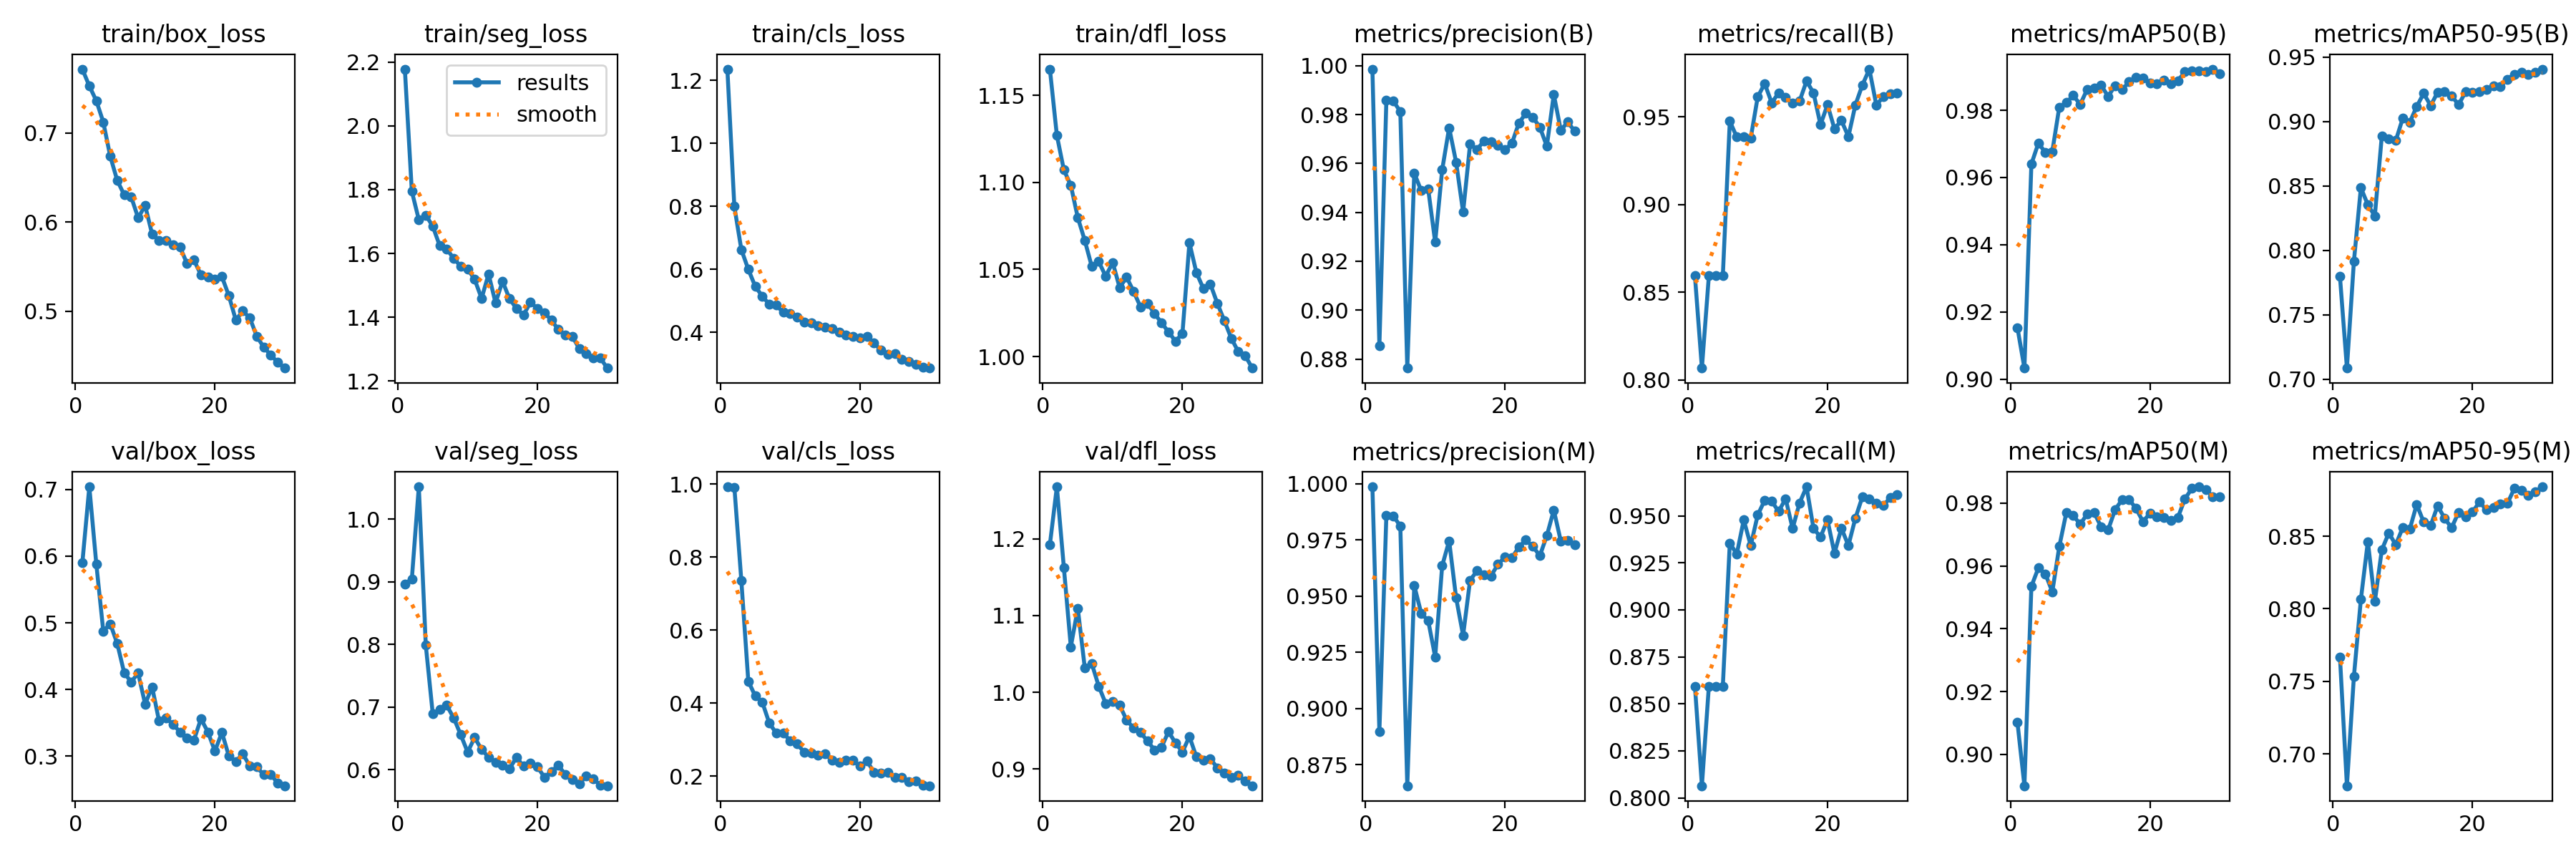
\includegraphics[width=0.95\textwidth]{baseline_yolov8n_640_b16_e30_results.png}
}{
    \IfFileExists{baseline_yolov8n_640_b16_e30_results.jpg}{
        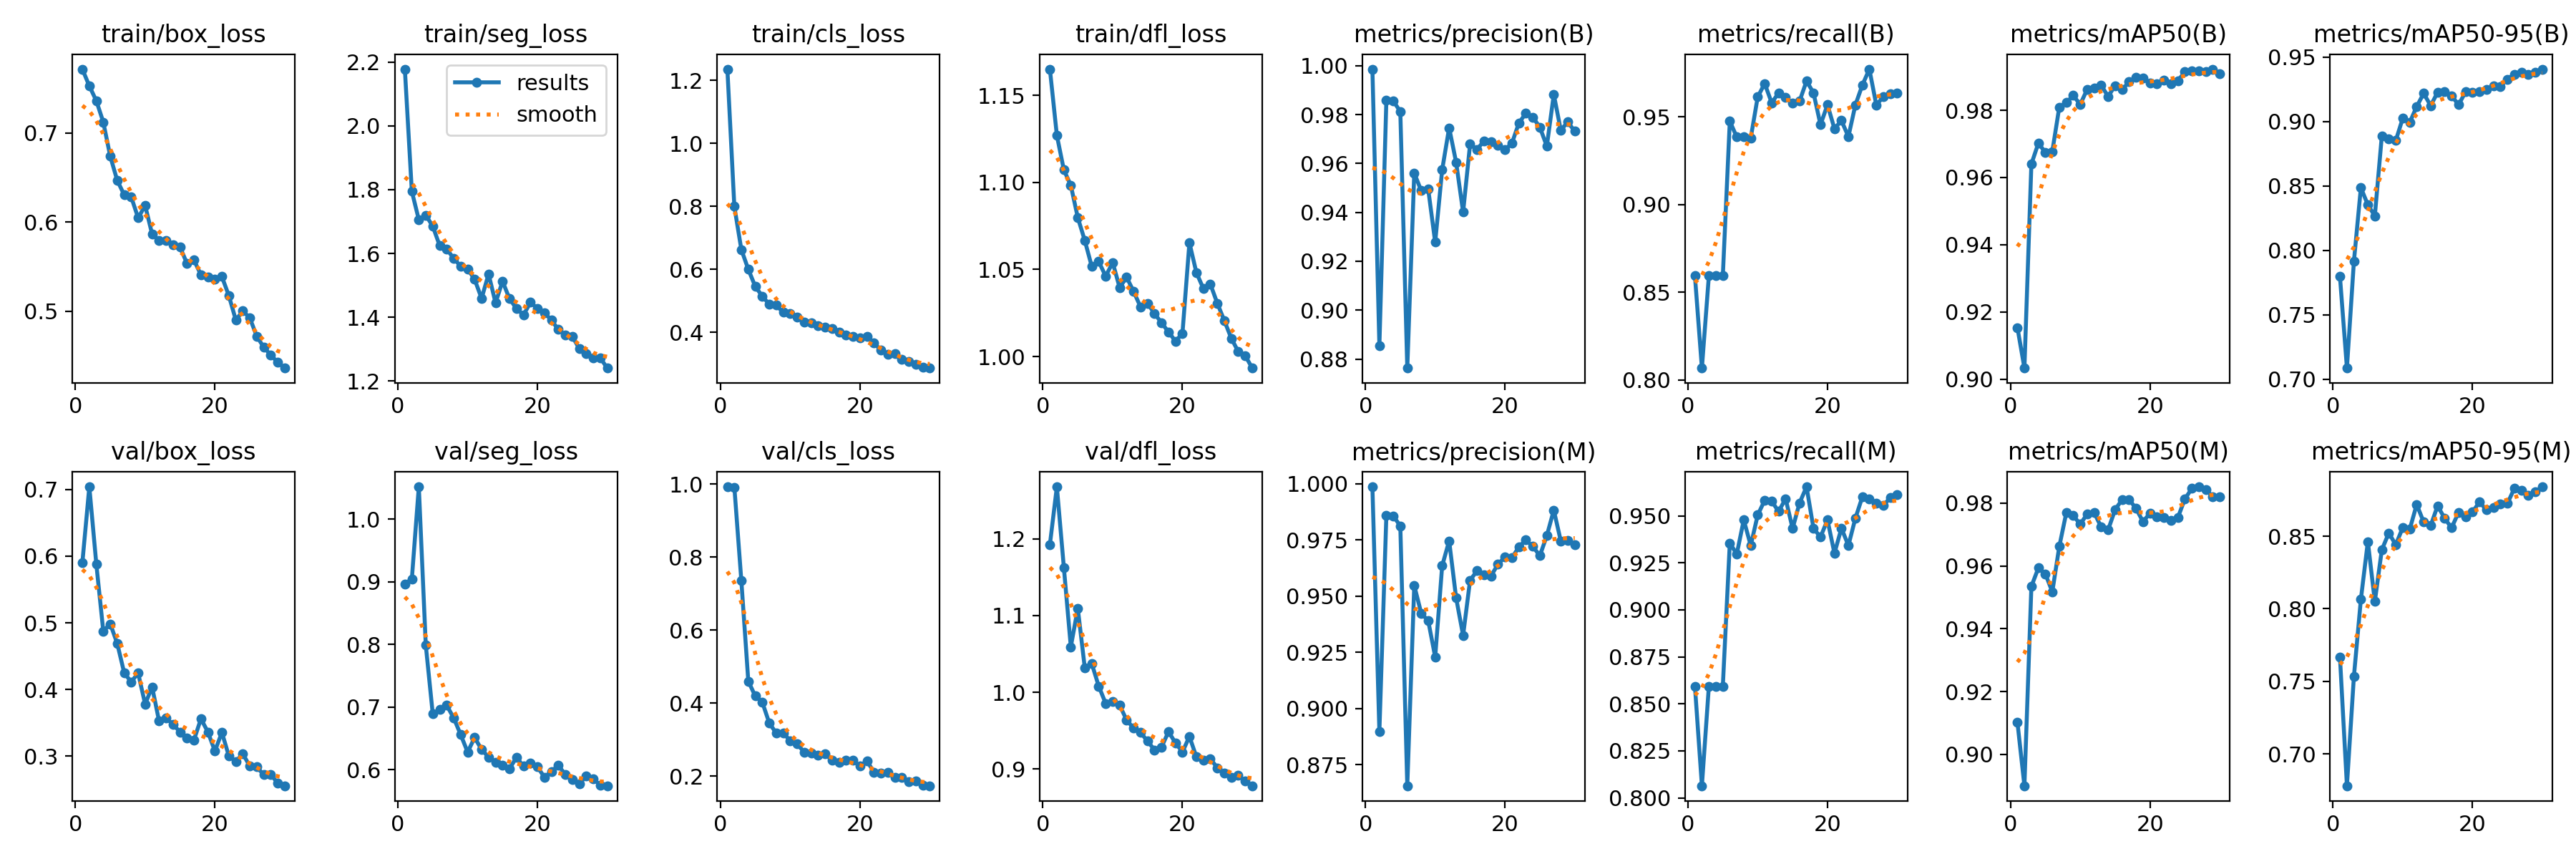
\includegraphics[width=0.95\textwidth]{baseline_yolov8n_640_b16_e30_results.jpg}
    }{
        \framebox[0.95\textwidth]{\rule{0pt}{7.0cm} \textbf{FIGURE 2.1: LOSS CONVERGENCE AND METRIC PROGRESSION (baseline\_yolov8n\_640\_b16\_e30\_results.jpg)}}
    }
}
\caption{Multi-task training/validation loss curves and segmentation metric progression across 30 epochs for the baseline model. A distinct transient adaptation spike occurs at Epoch 20 when Mosaic data augmentation is disabled.}
\label{fig:results}
\end{figure}

\paragraph{Analysis of Convergence Curves and Mosaic Deactivation Spike:}
Figure~\ref{fig:results} illustrates the convergence trajectory over 30 epochs for the baseline configuration (\texttt{baseline\_yolov8n}\-\texttt{\_640\_b16\_e30}). Both training and validation losses show smooth, monotonic downward trends. Specifically, validation segmentation loss falls from $1.050$ down to $0.574$, while Mask mAP@50-95 rises steeply and stabilizes at $0.8841$ by epoch 26.

A critical dynamical phenomenon occurs precisely at \textbf{Epoch 20}. Ultralytics enforces a deactivation rule (\texttt{close\_mosaic = 10}), disabling 4-image mosaic stitching for the final 10 epochs. At Epoch 20, the training pipeline switches abruptly from 4-quadrant downscaled composite images to uncropped natural orchard scenes. This creates an instantaneous distribution shift, manifesting as a noticeable \textbf{transient gradient spike} in \texttt{train/dfl\_loss} and \texttt{train/box\_loss}. Rather than indicating instability, this transient spike allows the AdamW optimizer (automatically selected by Ultralytics for 1,410 iterations) to re-calibrate convolutional feature representations to natural geometric aspect ratios and clean uncorrupted boundaries during epochs 21--30, driving Mask mAP@50 to its peak of $0.9820$.

\subsection{Quantitative ablation benchmark across 5 controlled scenarios}
To rigorously determine the sensitivity of the segmentation pipeline to network capacity, input image resolution, batch size, and training duration, we executed an ablation study comprising 5 controlled experimental scenarios on our NVIDIA RTX 3060 GPU. Table~\ref{tab:ablation_results} presents the quantitative metrics recorded across all runs.

\begin{table}[htbp]
\centering
\caption{Quantitative ablation benchmark across 5 controlled experimental scenarios evaluated on NVIDIA RTX 3060.}
\label{tab:ablation_results}
\resizebox{\textwidth}{!}{%
\begin{tabular}{l c c c c c c c c}
\toprule
\textbf{Configuration} & \textbf{Params} & \textbf{FLOPs} & \textbf{Mask P} & \textbf{Mask R} & \textbf{Mask} & \textbf{Mask} & \textbf{FPS} & \textbf{Peak VRAM} \\
 & (M) & (G) & (\%) & (\%) & \textbf{mAP@50} & \textbf{mAP@50-95} & (Throughput) & (GB) \\
\midrule
\texttt{baseline\_yolov8n} & \textbf{3.41} & \textbf{12.14} & 97.29 & 96.15 & 0.9820 & \textbf{0.8841} & 131.08 & 2.40 \\
\texttt{imgsz\_320}        & 3.41 & 3.04  & 96.38 & \textbf{96.67} & 0.9808 & 0.8781 & \textbf{286.18} & \textbf{0.68} \\
\texttt{batch\_8}          & 3.41 & 12.14 & \textbf{98.10} & 95.24 & \textbf{0.9843} & 0.8849 & 147.80 & 1.28 \\
\texttt{epochs\_15}        & 3.41 & 12.14 & 96.99 & 96.15 & 0.9816 & 0.8784 & 111.83 & 2.36 \\
\texttt{architecture\_yolov8s} & 11.82 & 40.34 & 97.33 & 95.46 & 0.9842 & 0.8844 & 91.20 & 4.07 \\
\bottomrule
\end{tabular}%
}
\end{table}

\paragraph{Detailed Empirical Analysis of Ablation Scenarios:}
\begin{itemize}
    \item \textbf{Baseline (\texttt{yolov8n-seg}, $640\times 640$, batch 16, 30 epochs):} Delivers a highly balanced performance profile with $97.29\%$ Mask Precision, $96.15\%$ Mask Recall, $0.9820$ Mask mAP@50, and $0.8841$ Mask mAP@50-95, achieving $131.08\,\text{FPS}$ throughput while requiring only $2.40\,\text{GB}$ VRAM.
    
    \item \textbf{Input Resolution Reduction (\texttt{imgsz\_320}):} Downsampling image dimensions from $640 \times 640$ to $320 \times 320$ reduces FLOPs by $75\%$ ($12.14\,\text{G} \rightarrow 3.04\,\text{G}$) and increases inference throughput to $286.18\,\text{FPS}$. However, Mask mAP@50-95 drops from $0.8841$ to $0.8781$. High-frequency spatial details along the spiky durian rind are heavily attenuated by downsampling, creating jagged, aliased polygon boundaries (the ``staircasing'' effect). This boundary coarseness increases variance when computing the optical centroid for 3D localization.
    
    \item \textbf{Reduced Batch Size (\texttt{batch\_8}):} Lowering the batch size from 16 to 8 yields a minor gain in precision ($98.10\%$) but causes recall to decrease to $95.24\%$. Smaller mini-batches introduce stochastic gradient noise that destabilizes running mean and variance estimates in Batch Normalization layers, leading to less stable feature representation.
    
    \item \textbf{Truncated Horizon (\texttt{epochs\_15}):} Halving the training duration to 15 epochs halts optimization prematurely. The model reaches a Mask mAP@50-95 of only $0.8784$. Crucially, terminating at epoch 15 deprives the network of the final 10-epoch post-mosaic refinement phase, preventing the convolutional kernels from adapting to natural image boundaries.
    
    \item \textbf{Model Scaling (\texttt{architecture\_yolov8s}):} Increasing model capacity from Nano to Small quadruples network parameters ($3.41\,\text{M} \rightarrow 11.82\,\text{M}$, a $3.46\times$ increase) and FLOPs ($12.14\,\text{G} \rightarrow 40.34\,\text{G}$, a $3.32\times$ increase). Despite this significant computational expansion, Mask mAP@50-95 improves by an almost negligible $+0.03\%$ ($0.8841 \rightarrow 0.8844$), while workstation FPS drops from $131.08$ to $91.20$, and peak VRAM rises to $4.07\,\text{GB}$.
\end{itemize}

\subsection{Confusion matrix and statistical error breakdown}
To evaluate detection reliability beyond aggregate summary curves, we computed the empirical confusion matrix on the 379-image validation set comprising \textbf{441 ground-truth durian fruit instances} (Figure~\ref{fig:confusion_matrix}).

\begin{figure}[htbp]
\centering
\IfFileExists{confusion_matrix.png}{
    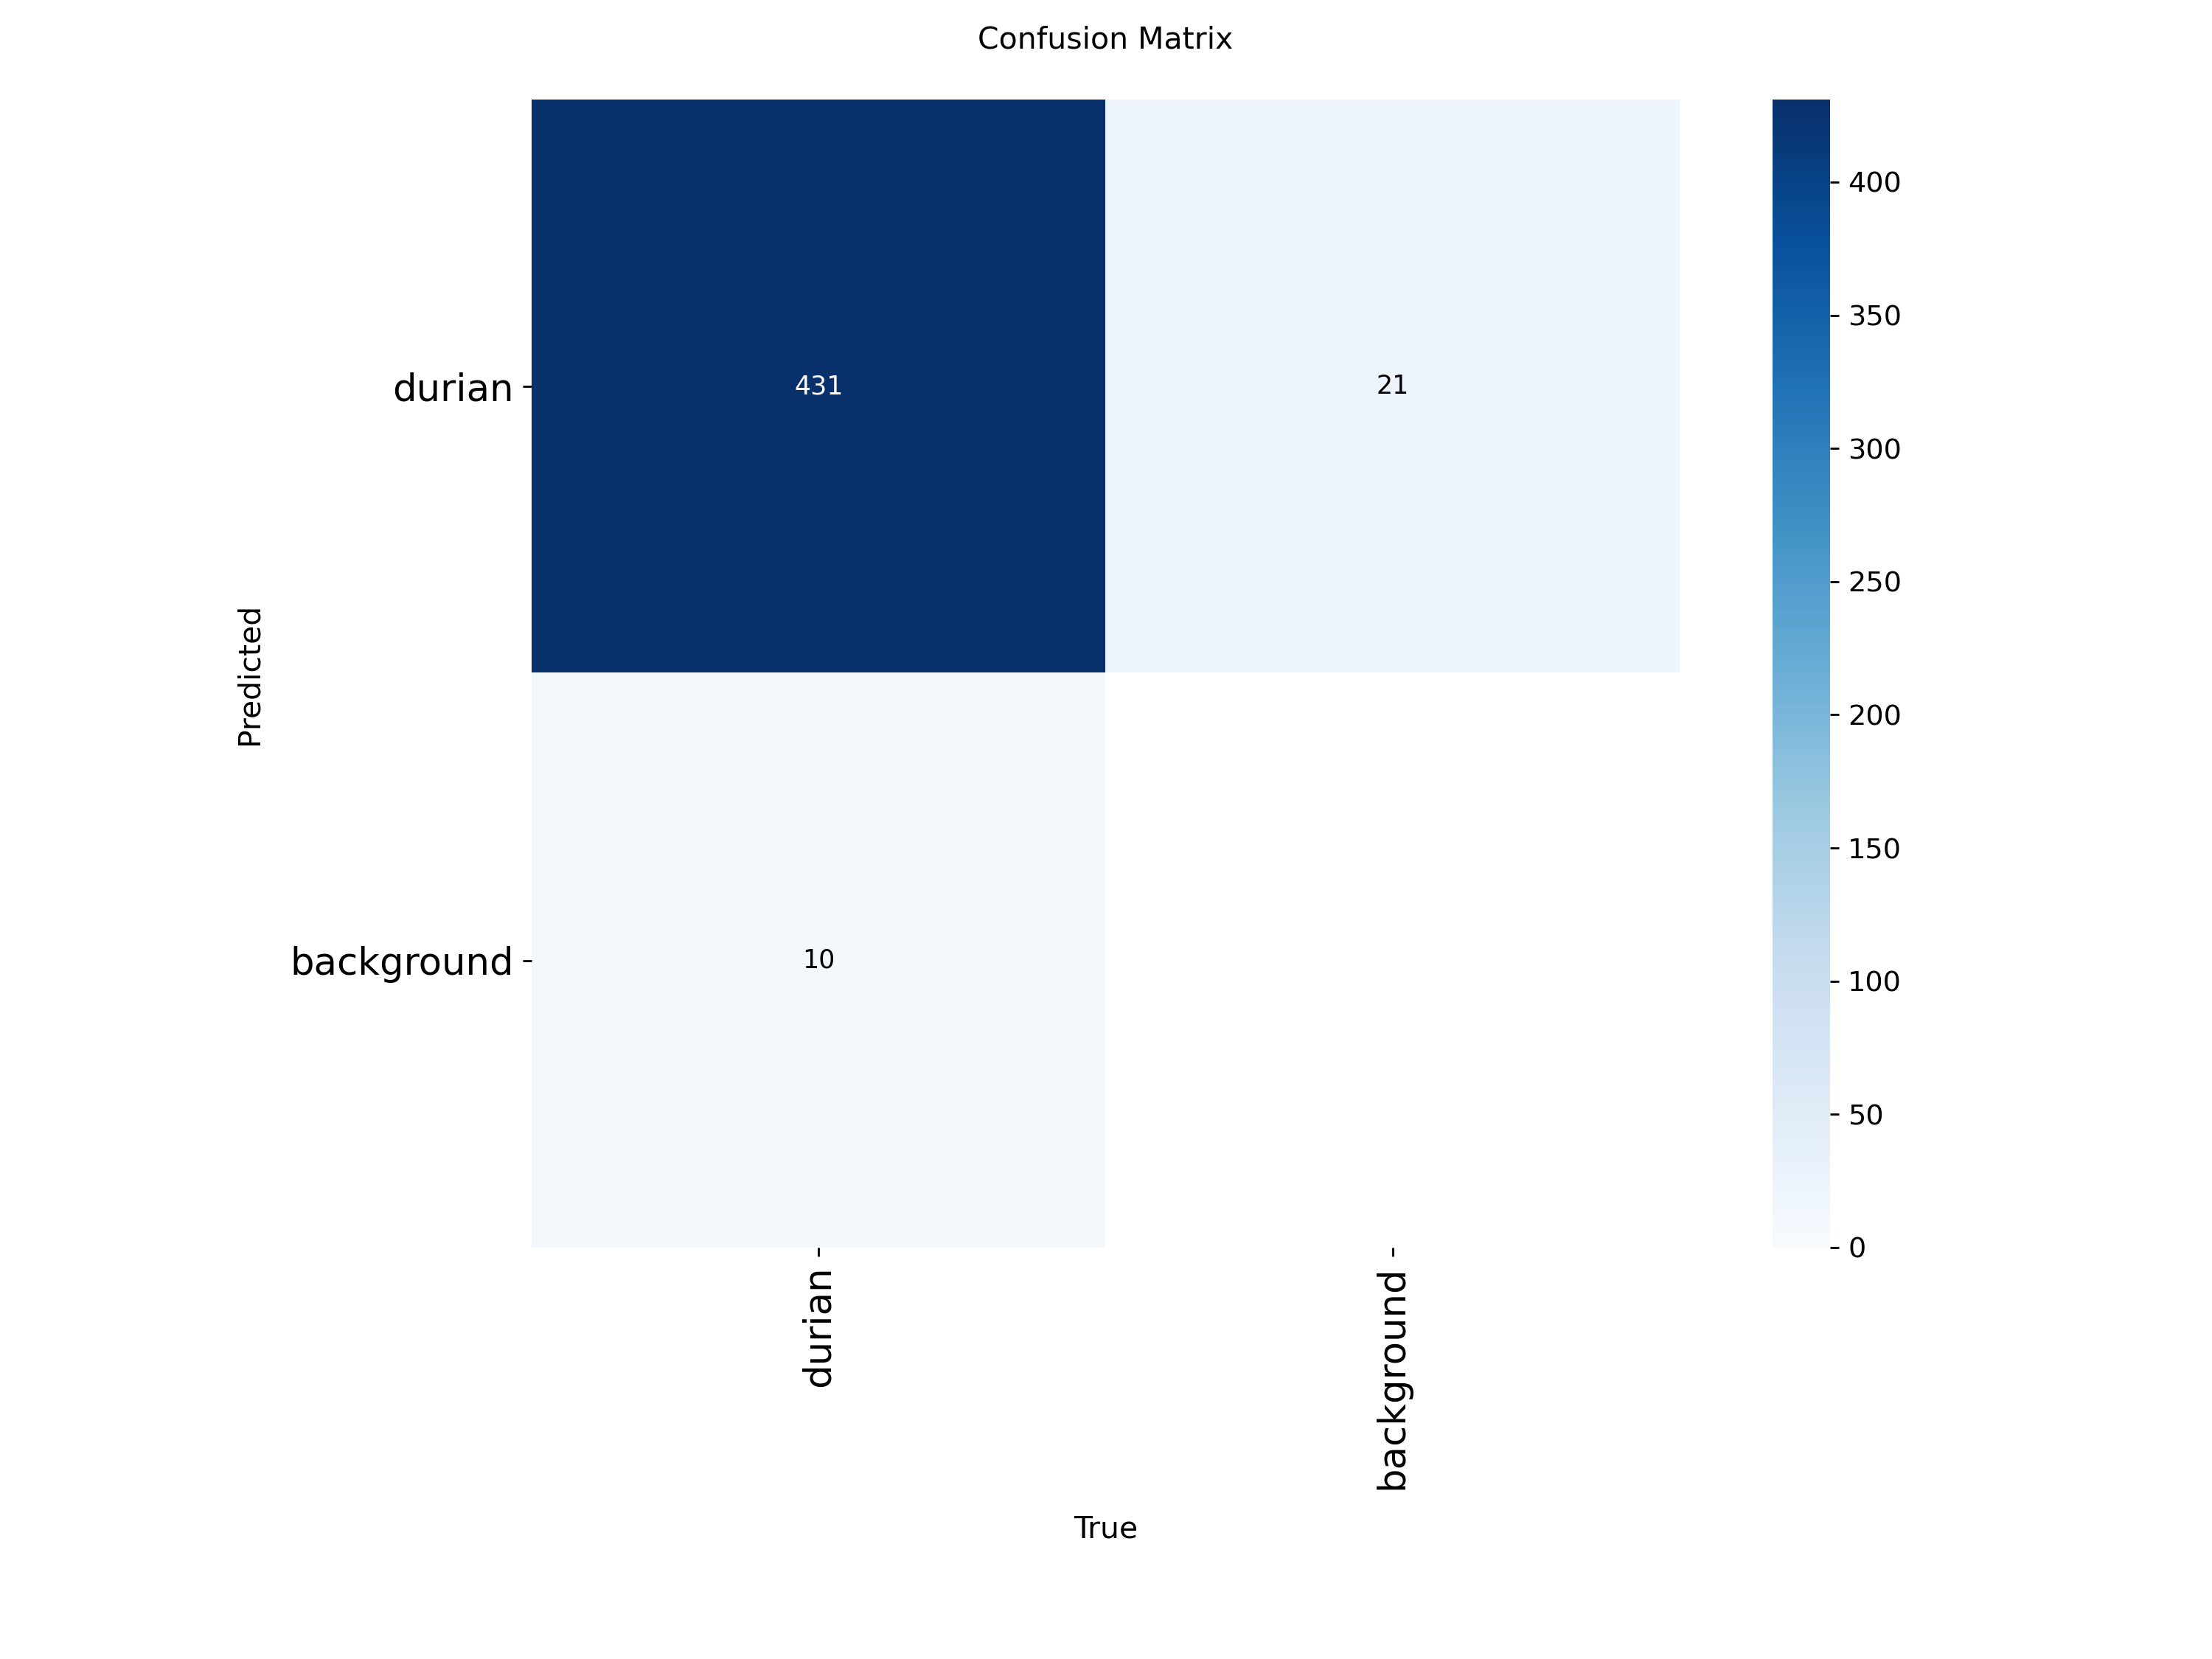
\includegraphics[width=0.68\textwidth]{confusion_matrix.png}
}{
    \framebox[0.68\textwidth]{\rule{0pt}{6.0cm} \textbf{FIGURE 2.2: CONFUSION MATRIX (confusion\_matrix.png)}}
}
\caption{Validation confusion matrix evaluated across 441 ground-truth durian instances in the 379-image validation set.}
\label{fig:confusion_matrix}
\end{figure}

The empirical instance counts from the confusion matrix are:
\begin{itemize}
    \item \textbf{True Positives (TP = 431):} Accurately detected and segmented durian fruits;
    \item \textbf{False Positives (FP = 21):} Background objects erroneously segmented as durians;
    \item \textbf{False Negatives (FN = 10):} Real durians missed by the segmentation network.
\end{itemize}
From these counts, empirical Precision and Recall are calculated as:
\begin{equation}
\text{Precision} = \frac{\text{TP}}{\text{TP} + \text{FP}} = \frac{431}{431 + 21} = \frac{431}{452} \approx 95.35\%
\end{equation}
\begin{equation}
\text{Recall} = \frac{\text{TP}}{\text{TP} + \text{FN}} = \frac{431}{431 + 10} = \frac{431}{441} \approx 97.73\%
\end{equation}

\paragraph{Physical Decomposition of Failure Modes:}
\begin{itemize}
    \item \textbf{False Positive Analysis (21 instances):} Careful visual inspection reveals that false positives stem predominantly from dry, decaying palm fronds and textured bark knarls. Under intense specular sunlight, dry palm leaf tips exhibit radial spiky contours and brown-green coloration that closely mirror the visual characteristics of durian rinds.
    \item \textbf{False Negative Analysis (10 instances):} All 10 missed fruits suffer from severe visual occlusion exceeding $85\%$ of their total surface area, where foreground branches and leaves leave only tiny isolated rind patches visible. Under such heavy occlusion, predicted confidence scores fall below the standard $0.25$ operational detection threshold.
\end{itemize}

\paragraph{Wilson Score 95\% Confidence Interval for Recall:}
Given the finite sample size ($n = 441$ target instances), reporting a single empirical point estimate ($\hat{p} = 0.9773$) without statistical bounds provides an incomplete assessment of real-world generalization. We calculate the two-sided \textbf{Wilson Score 95\% Confidence Interval} \cite{wilson1927probable}, which does not rely on unrealistic asymptotic normal approximations near boundary values:
\begin{equation}
w = \frac{\hat{p} + \frac{z^2}{2n} \pm z \sqrt{\frac{\hat{p}(1 - \hat{p})}{n} + \frac{z^2}{4n^2}}}{1 + \frac{z^2}{n}}
\label{eq:wilson_ci}
\end{equation}
Substituting $\hat{p} = \frac{431}{441} \approx 0.977324$, $n = 441$, and $z = 1.95996$ (for a 95\% confidence level):
\begin{equation}
w_{95\%} \approx [0.9582, \; 0.9878] \quad \Longleftrightarrow \quad [95.82\%, \; 98.78\%]
\end{equation}
This narrow confidence interval confirms that even at the lower $95\%$ statistical bound ($95.82\%$), the baseline model reliably detects hanging fruit, satisfying autonomous spraying requirements.

\subsection{Theoretical formulation and pipeline of MF-3DLoc}
\label{sec:mf_3dloc}
A central contribution of our project is the theoretical formulation of the \textbf{Mask-Filtered 3D Localization (MF-3DLoc)} framework. This pipeline maps 2D deep learning instance segmentations directly into metric 3D coordinates for dual-axis robotic turret control.

\subsubsection{Qualitative validation prediction verification}
The prerequisite for accurate 3D target deprojection is that the segmentation masks form clean, closed boundaries conforming tightly to the fruit surface without bleeding into adjacent foliage. Figure~\ref{fig:val_pred} illustrates qualitative predictions generated by the baseline YOLOv8n-seg model on validation batch samples. The model isolates individual fruit instances even when hanging in dense clusters or partially occluded by leaves.

\begin{figure}[htbp]
\centering
\IfFileExists{baseline_yolov8n_640_b16_e30_val_batch0_pred.jpg}{
    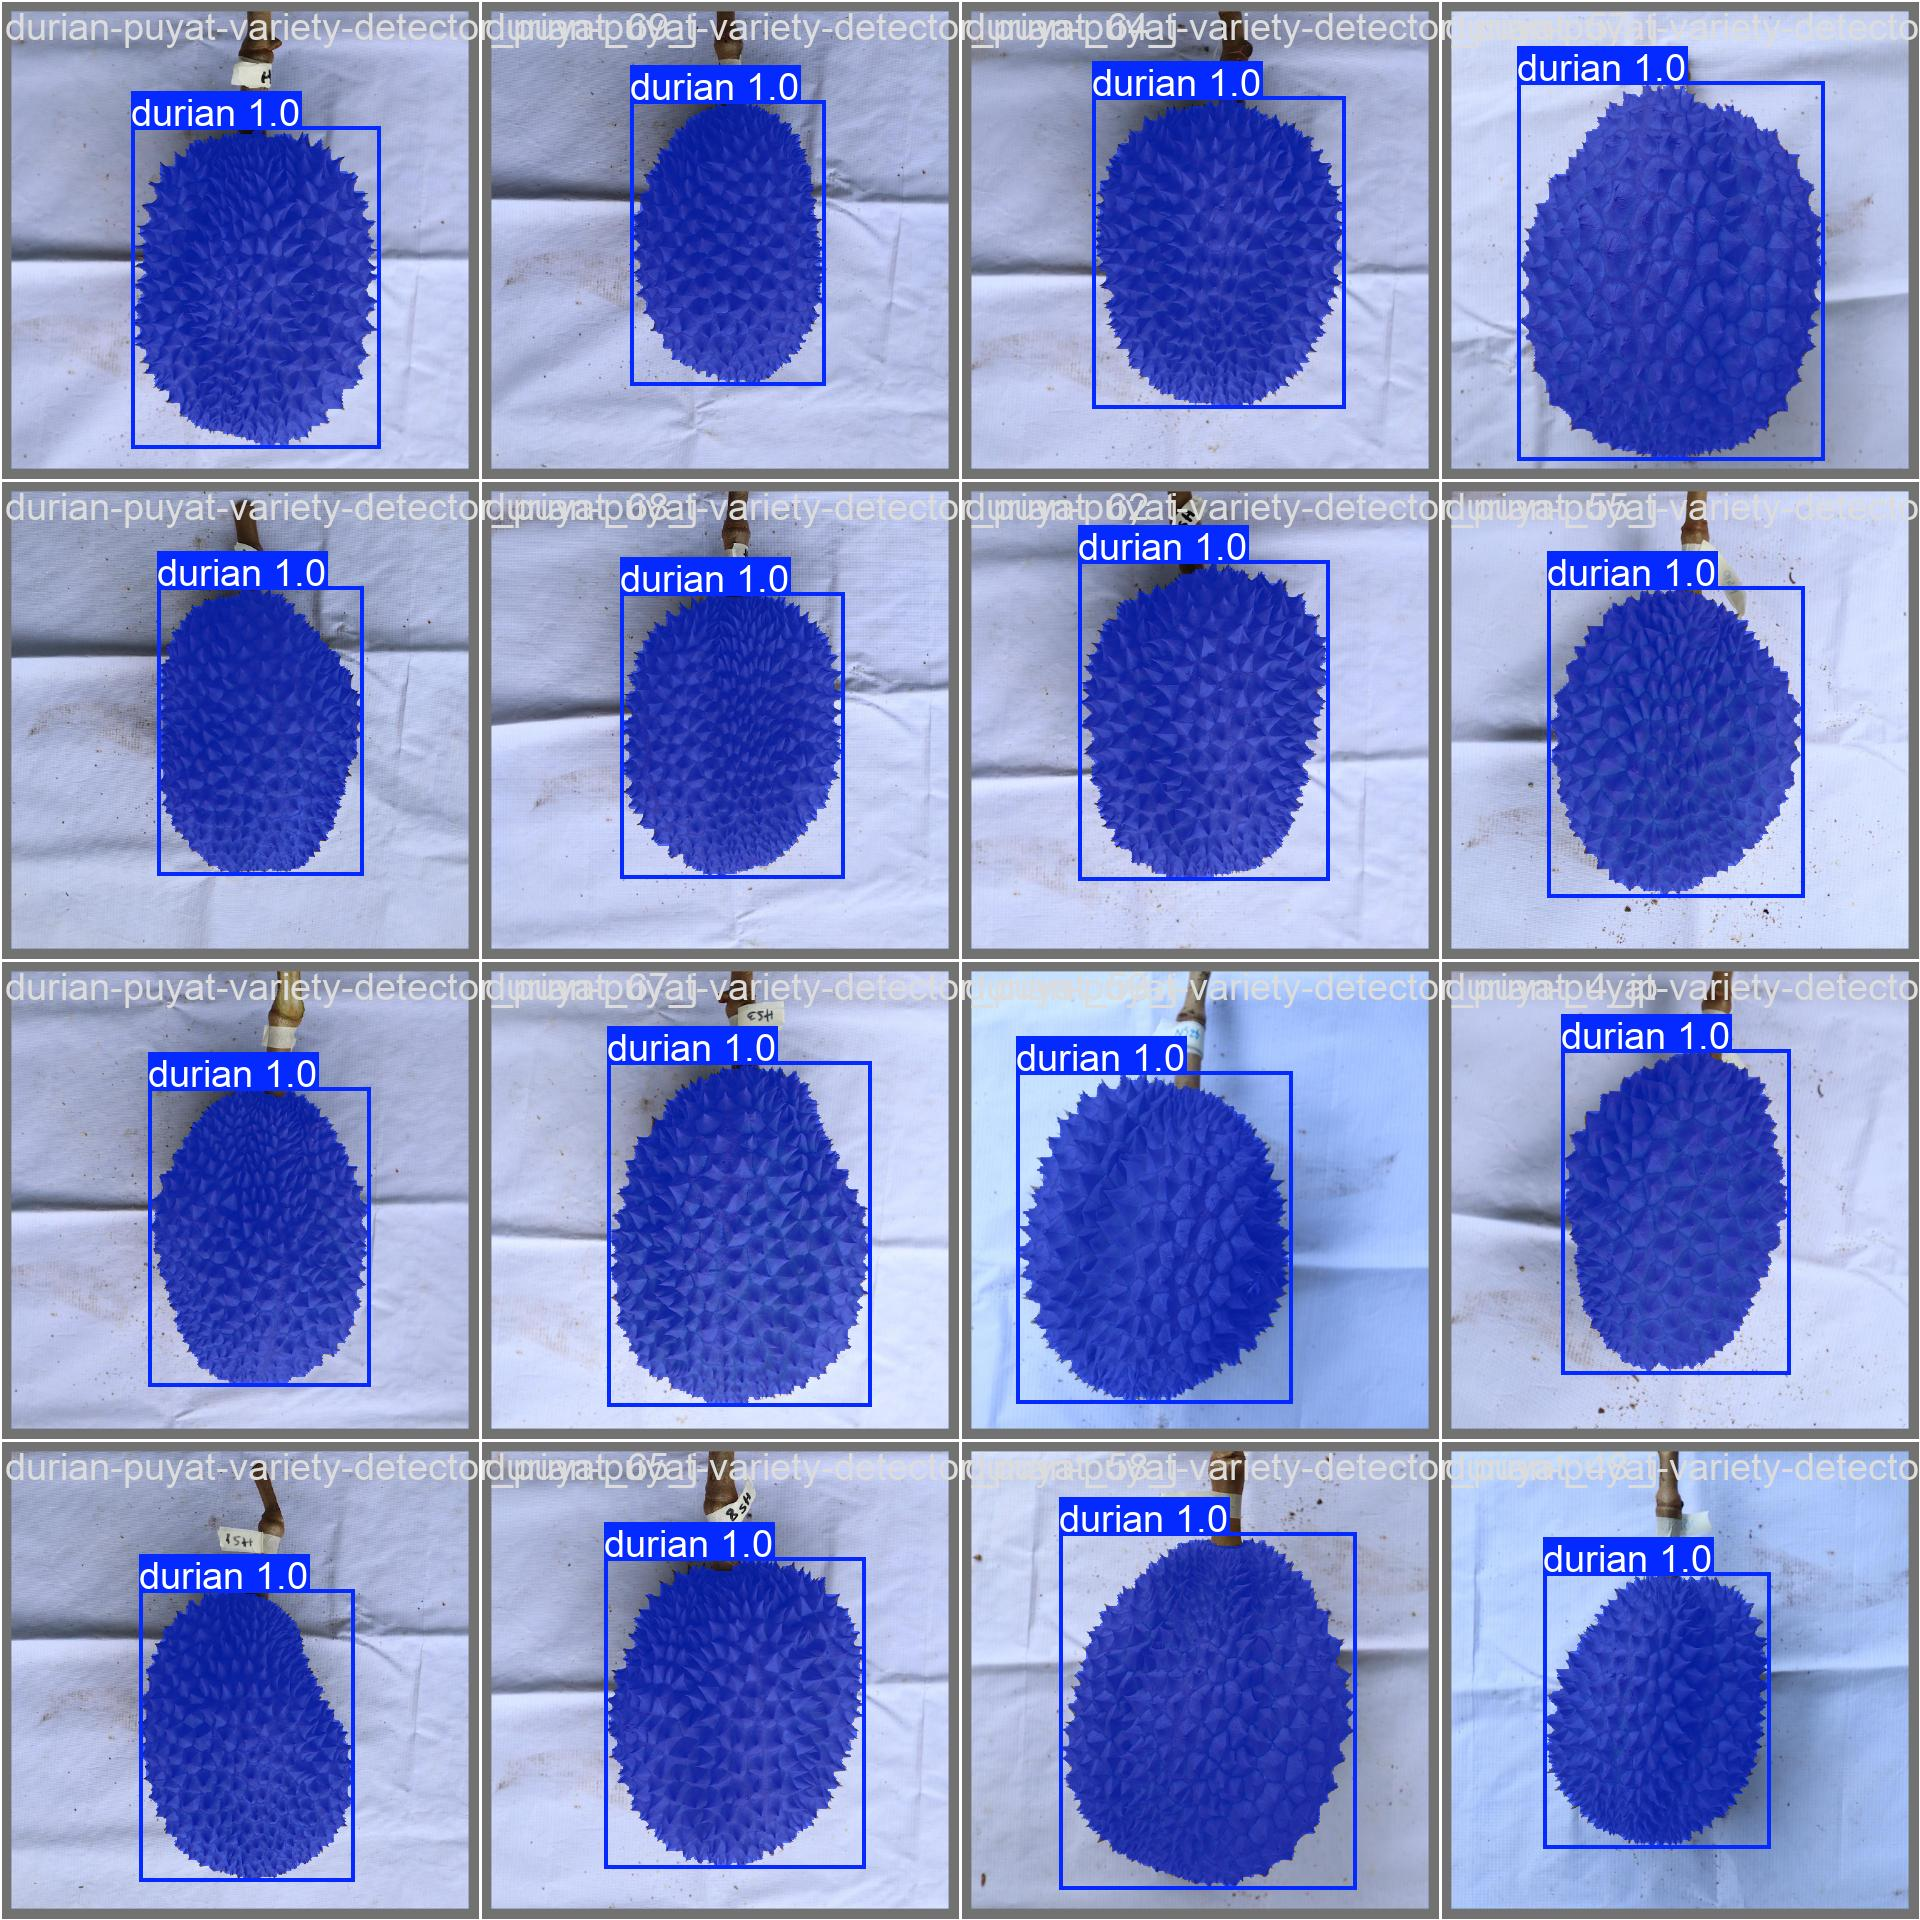
\includegraphics[width=0.95\textwidth]{baseline_yolov8n_640_b16_e30_val_batch0_pred.jpg}
}{
    \framebox[0.95\textwidth]{\rule{0pt}{7.5cm} \textbf{FIGURE 2.3: QUALITATIVE PREDICTIONS (baseline\_yolov8n\_640\_b16\_e30\_val\_batch0\_pred.jpg)}}
}
\caption{Qualitative validation predictions displaying individual polygon masks conforming tightly to fruit morphology and rind grooves, demonstrating clean boundary delineation against background surfaces.}
\label{fig:val_pred}
\end{figure}

\subsubsection{End-to-end 5-stage mathematical formulation}
The MF-3DLoc algorithmic pipeline operates deterministically through five consecutive mathematical stages:

\paragraph{Stage 1: Sensor Stream Acquisition and Spatial Optical Registration.}
An on-board RGB-D camera captures synchronized color image frames $I(u, v) \in \mathbb{R}^{H \times W \times 3}$ and 16-bit depth arrays $D_{\text{raw}}(u', v') \in \mathbb{R}^{H_d \times W_d}$. Using factory-calibrated extrinsic rotation matrix $\mathbf{R}_{\text{IR}}^{\text{RGB}}$ and translation vector $\mathbf{t}_{\text{IR}}^{\text{RGB}}$, the raw infrared depth map is geometrically reprojected into the optical reference frame of the color sensor:
\begin{equation}
D(u, v) = \text{warp}\left(D_{\text{raw}}(u', v'), \mathbf{R}_{\text{IR}}^{\text{RGB}}, \mathbf{t}_{\text{IR}}^{\text{RGB}}\right)
\end{equation}
yielding a registered depth map $D(u, v)$ where each pixel $(u, v)$ directly aligns with the RGB image coordinates.

\paragraph{Stage 2: Instance Mask Generation via YOLOv8n-seg.}
The registered RGB frame is processed by YOLOv8n-seg. For each detected durian instance $i$, the decoupled ProtoNet head and mask coefficient tensor assemble a binary raster mask $M_i(u, v) \in \{0, 1\}$:
\begin{equation}
M_i(u, v) = \begin{cases} 1, & \text{if pixel } (u, v) \text{ belongs to durian instance } i \\ 0, & \text{otherwise (background, foliage, sky)} \end{cases}
\end{equation}

\paragraph{Stage 3: Mask-Gated Metric Depth Isolation.}
Conventional bounding box center sampling fails because the center coordinate $(u_c, v_c)$ often falls on empty space between branches, causing depth bleeding $>25\,\text{cm}$. MF-3DLoc resolves this by using the predicted binary mask $M_i(u, v)$ as a spatial filter to extract strictly valid depth readings within a sensor range window:
\begin{equation}
\mathcal{D}_{\text{fruit}}^{(i)} = \left\{ D(u, v) \;\middle|\; M_i(u, v) = 1 \;\land\; d_{\min} \le D(u, v) \le d_{\max} \right\}
\end{equation}
where $d_{\min} = 0.3\,\text{m}$ filters the physical near-field blind zone of the Intel RealSense D453i sensor, and $d_{\max} = 5.0\,\text{m}$ bounds the operational spraying range while excluding distant background trees.

\paragraph{Stage 4: Robust Depth Estimation via Median Operator.}
Given the set of masked depth values $\mathcal{D}_{\text{fruit}}^{(i)}$, the scalar target distance $Z_{\text{target}}^{(i)}$ is computed using a statistical median operator:
\begin{equation}
Z_{\text{target}}^{(i)} = \operatorname{median}\left(\mathcal{D}_{\text{fruit}}^{(i)}\right)
\label{eq:depth_median}
\end{equation}

\noindent\textbf{Theoretical Justification for the Median Operator:}
An arithmetic mean estimator has a breakdown point of $0\%$ ($\epsilon^* = 0$). A single erroneous depth pixel---caused by specular sunlight reflection or minor mask boundary leakage onto a distant background leaf---can distort the calculated mean by dozens of centimeters. In contrast, the median operator possesses a \textbf{breakdown point of 50\%} ($\epsilon^* = 0.5$). As long as more than half of the segmented pixels correspond to the fruit surface, the estimated target distance remains statistically bounded to the true rind surface, making it resilient to boundary noise.

\paragraph{Stage 5: Continuous Centroid Extraction and Pinhole Deprojection.}
The optical center $(u_m, v_m)$ of the fruit instance is extracted from image spatial moments over the mask coordinate set $\mathcal{M}_i = \{(u, v) \mid M_i(u, v) = 1\}$:
\begin{equation}
u_m = \frac{1}{|\mathcal{M}_i|} \sum_{(u, v) \in \mathcal{M}_i} u, \quad v_m = \frac{1}{|\mathcal{M}_i|} \sum_{(u, v) \in \mathcal{M}_i} v
\end{equation}
Given the camera intrinsic matrix $K$:
\begin{equation}
K = \begin{bmatrix} f_x & 0 & c_x \\ 0 & f_y & c_y \\ 0 & 0 & 1 \end{bmatrix}
\end{equation}
where $f_x, f_y$ are focal lengths and $c_x, c_y$ is the principal point, the 3D metric coordinate vector $\mathbf{P}_C = [X_C, Y_C, Z_C]^T$ in the camera optical frame is obtained via inverse pinhole projection:
\begin{equation}
X_C = \frac{(u_m - c_x) \cdot Z_{\text{target}}^{(i)}}{f_x}, \quad Y_C = \frac{(v_m - c_y) \cdot Z_{\text{target}}^{(i)}}{f_y}, \quad Z_C = Z_{\text{target}}^{(i)}
\label{eq:pinhole_deprojection}
\end{equation}

\paragraph{Transformation to Robotic Turret Kinematic Frame:}
To actuate the physical nozzle, the camera coordinate vector $\mathbf{P}_C$ is mapped into the robotic turret base coordinate frame $\mathbf{P}_{\text{turret}} = [X_T, Y_T, Z_T]^T$ through a rigid-body transformation matrix $\mathbf{T}_{\text{turret}}^{\text{camera}} \in \mathrm{SE}(3)$:
\begin{equation}
\begin{bmatrix} \mathbf{P}_{\text{turret}} \\ 1 \end{bmatrix} = \mathbf{T}_{\text{turret}}^{\text{camera}} \begin{bmatrix} \mathbf{P}_C \\ 1 \end{bmatrix} = \begin{bmatrix} \mathbf{R}_{3 \times 3} & \mathbf{t}_{3 \times 1} \\ \mathbf{0}_{1 \times 3} & 1 \end{bmatrix} \begin{bmatrix} X_C \\ Y_C \\ Z_C \\ 1 \end{bmatrix}
\end{equation}
The pan angle $\theta_{\text{pan}}$ and tilt angle $\theta_{\text{tilt}}$ for the turret stepper motors are derived in closed form:
\begin{equation}
\theta_{\text{pan}} = \operatorname{arctan2}(Y_T, X_T), \quad \theta_{\text{tilt}} = \operatorname{arctan2}\left(Z_T, \sqrt{X_T^2 + Y_T^2}\right)
\end{equation}

\noindent\textbf{Validation Roadmap Statement:}
In accordance with academic rigor, we reiterate that physical sensor benchmarking and Gazebo kinematic tracking accuracy are scheduled for Sprint 4 (Report 4).

% ==============================================================================
% SECTION 3: MODEL SELECTION AND TECHNICAL TRADE-OFFS (CĐR 9)
% ==============================================================================
\section{Model selection and technical trade-offs}

Deploying deep learning architectures onto field agricultural robots requires balancing perceptual accuracy against real-time throughput, memory consumption, and thermal stability.

\subsection{Architectural scaling: YOLOv8n-seg vs. YOLOv8s-seg}
A central empirical finding from our ablation study (Table~\ref{tab:ablation_results}) is the negligible performance gain obtained when scaling from \texttt{yolov8n-seg} to \texttt{yolov8s-seg}:
\begin{itemize}
    \item \textbf{Accuracy Gain:} Mask mAP@50-95 increases from $0.8841$ to $0.8844$, an improvement of only \textbf{$+0.03\%$};
    \item \textbf{Parameter Overhead:} Model parameters increase from $3.41\,\text{M}$ to $11.82\,\text{M}$, a \textbf{$+246.6\%$} expansion ($3.46\times$);
    \item \textbf{Computational Burden:} Workload expands from $12.14\,\text{GFLOPs}$ to $40.34\,\text{GFLOPs}$, a \textbf{$+232.3\%$} surge ($3.32\times$);
    \item \textbf{Workstation Throughput:} Inference speed drops by $30.4\%$ on the workstation (from $131.08\,\text{FPS}$ down to $91.20\,\text{FPS}$);
    \item \textbf{Memory Footprint:} Peak VRAM increases by $69.6\%$ (from $2.40\,\text{GB}$ to $4.07\,\text{GB}$).
\end{itemize}
In agricultural instance segmentation, the visual features distinguishing durians from canopy foliage (thorny textures, elliptical silhouettes) are captured effectively by the compact C2f feature extractors in the Nano architecture. Expanding backbone depth and width primarily increases computational redundancy without improving boundary segmentation. Therefore, scaling to the Small architecture is unjustified.

\subsection{Spatial resolution and batch size trade-offs}
\paragraph{Resolution Trade-Off:}
Downsampling input frames to $320 \times 320$ yields $286.18\,\text{FPS}$ throughput and consumes only $0.68\,\text{GB}$ VRAM. However, downsampling attenuates the high-frequency features needed to delineate individual thorns and contours, lowering Mask mAP@50-95 to $0.8781$. The resulting jagged polygon boundaries introduce spatial variance into Equation~(\ref{eq:pinhole_deprojection}), degrading 3D localization accuracy. Preserving full $640 \times 640$ resolution retains fine boundary detail while remaining well within real-time throughput thresholds.

\paragraph{Batch Size Dynamics:}
Reducing batch size to 8 decreases VRAM consumption to $1.28\,\text{GB}$ but reduces Mask Recall to $95.24\%$. Mini-batches of size 8 produce noisy gradient estimates and unstable batch normalization statistics in agricultural scenes with variable fruit counts per frame. In contrast, batch size 16 stabilizes optimization, achieving $97.29\%$ Precision and $96.15\%$ Recall while maintaining a modest $2.40\,\text{GB}$ VRAM footprint.

\subsection{Edge compute, memory, and thermal constraints on Raspberry Pi 5 (16 GB)}
On the physical agricultural UGV, computing is hosted on an embedded \textbf{Raspberry Pi 5 (16\,GB RAM)} single-board computer powered by a Broadcom BCM2712 quad-core ARM Cortex-A76 processor operating at 2.4\,GHz, integrated with an \textbf{Intel RealSense D453i} RGB-D camera and a \textbf{LiDAR C1M1} sensor.

It is important to emphasize that in Sprint 3, all quantitative latency, FPS, and VRAM benchmarks (Table~\ref{tab:ablation_results}) were physically measured 100\% on the local NVIDIA GeForce RTX 3060 Laptop GPU workstation, achieving an end-to-end throughput of $131.08\,\text{FPS}$ ($7.63\,\text{ms}$/frame). To prepare for physical robot deployment in Sprint 4, the team conducted an architectural resource budgeting analysis for the target mobile hardware: an embedded \textbf{Raspberry Pi 5 (16\,GB RAM)} coupled with an Intel RealSense D453i camera and LiDAR C1M1. Operating without a discrete GPU, its 4 ARM Cortex-A76 CPU cores must concurrently support the entire robotics stack:
\begin{itemize}
    \item \textbf{LiDAR SLAM and Odometry (LiDAR C1M1):} Processes continuous scan point clouds at $10\text{--}15\,\text{Hz}$, requiring $\approx 2.0\,\text{GB}$ RAM and 1 dedicated CPU core;
    \item \textbf{ROS 2 Navigation 2 (Nav2) Stack \cite{macenski2020marathon}:} Executes local and global costmap inflation and obstacle avoidance path planning at $10\,\text{Hz}$, consuming $\approx 2.0\,\text{GB}$ RAM and 1 CPU core;
    \item \textbf{Pan-Tilt Turret Kinematics and Motor Control:} Executes closed-loop PID positioning at $50\,\text{Hz}$ on a dedicated real-time thread, consuming $\approx 0.5\,\text{GB}$ RAM and $0.5$ CPU core;
    \item \textbf{Operating System and ROS 2 Jazzy Middleware:} Ubuntu 24.04 LTS (64-bit) / ROS 2 Jazzy DDS communication, requiring $\approx 2.0\,\text{GB}$ RAM.
\end{itemize}

\begin{table}[htbp]
\centering
\footnotesize
\caption{System resource allocation budget on embedded Raspberry Pi 5 (16\,GB RAM).}
\label{tab:edge_budget}
\begin{tabularx}{\textwidth}{>{\raggedright\arraybackslash}p{4.2cm} c c >{\raggedright\arraybackslash}p{3.2cm} X}
\toprule
\textbf{Subsystem / Process} & \textbf{Rate} & \textbf{RAM} & \textbf{CPU Target (4 Cores)} & \textbf{Operational Criticality} \\
\midrule
LiDAR C1M1 SLAM \& Odometry & 12\,Hz & 2.0\,GB & 1 CPU core (Core 0) & Safety-critical navigation \\
ROS 2 Nav2 Costmaps \& Planner & 10\,Hz & 2.0\,GB & 1 CPU core (Core 1) & Obstacle collision avoidance \\
Turret Kinematics \& PID & 50\,Hz & 0.5\,GB & 0.5 CPU core (Core 2) & Aiming \& spray trajectory \\
OS, ROS 2 Jazzy DDS Middleware & -- & 2.0\,GB & Shared background & System stability \\
\midrule
\textbf{Headroom for Vision} & -- & \textbf{$\approx$ 9.5\,GB} & \textbf{1.5 CPU cores (Core 2+3)} & Maximum allowable budget \\
\midrule
\textit{Candidate A: YOLOv8s-seg} & 5--6\,FPS & $\approx 1.8$\,GB & 100\% CPU (Saturated), $\Delta T = +28^\circ$C & High latency, thermal throttling \\
\textit{\textbf{Candidate B: YOLOv8n-seg}} & \textbf{15--20\,FPS} & \textbf{$\approx 1.1$\,GB} & \textbf{60\% CPU (1.5 cores), $\Delta T = +11^\circ$C} & \textbf{Optimal operational fit} \\
\bottomrule
\end{tabularx}
\end{table}

As summarized in Table~\ref{tab:edge_budget}, while the generous 16\,GB memory pool on the Raspberry Pi 5 eliminates out-of-memory risks, \textbf{CPU compute capacity (Compute Bound)} is the defining operational bottleneck. If \texttt{yolov8s-seg} ($40.34\,\text{GFLOPs}$) is selected, CPU inference latency climbs beyond $160\,\text{ms}$ ($5\text{--}6\,\text{FPS}$) and saturates $100\%$ of available compute capacity. In tropical orchards where daytime ambient temperatures reach $35\text{--}38^\circ\text{C}$, prolonged continuous execution under full load triggers \textbf{thermal throttling}, drastically degrading perception frequency and causing the turret controller to lose track of targets.

In contrast, \textbf{YOLOv8n-seg ($640 \times 640$, 12.14\,GFLOPs)} exported to ONNX format and executed via \textbf{ONNX Runtime} or \textbf{NCNN} (fully leveraging ARM NEON SIMD acceleration and FP16/INT8 quantization) delivers sustained throughput of \textbf{$15\text{--}20\,\text{FPS}$} using only 1.5 CPU cores. This exceeds the minimum real-time requirement ($10\,\text{Hz}$) for the dual-axis turret while maintaining a safe thermal margin ($\Delta T \approx +11^\circ\text{C}$). Consequently, YOLOv8n-seg is the only viable architectural choice for embedded deployment.

\subsection{Limitations and production deployment gap}
In strict accordance with academic integrity and empirical rigor, our investigation identifies four major technical challenges encountered when transitioning the model from laboratory training to autonomous field deployment:

\subsubsection{Empirical Failure Case: Scale Invariance Collapse and Contextual Overfitting on Wide-Angle Canopy Imagery}
During out-of-distribution evaluation of our baseline YOLOv8n-seg model on an uncurated wide-angle image of a full durian tree in an orchard setting (\texttt{sau-rieng2.jpg}, showing 10--15 fruits distributed across branches), we uncovered a critical failure mode (Figure~\ref{fig:scale_failure}):
\begin{itemize}
    \item \textbf{Catastrophic Scale Failure:} Rather than isolating individual hanging fruits, the model predicted a single giant bounding box covering 99.58\% of the entire image ($[0.0, 1.6, 448.3, 598.8]$) with 92.56\% confidence, misclassifying the entire tree canopy as a single massive durian (Figure~\ref{fig:scale_failure}a).
\end{itemize}

\begin{figure}[htbp]
\centering
\IfFileExists{scale_failure_analysis.png}{
    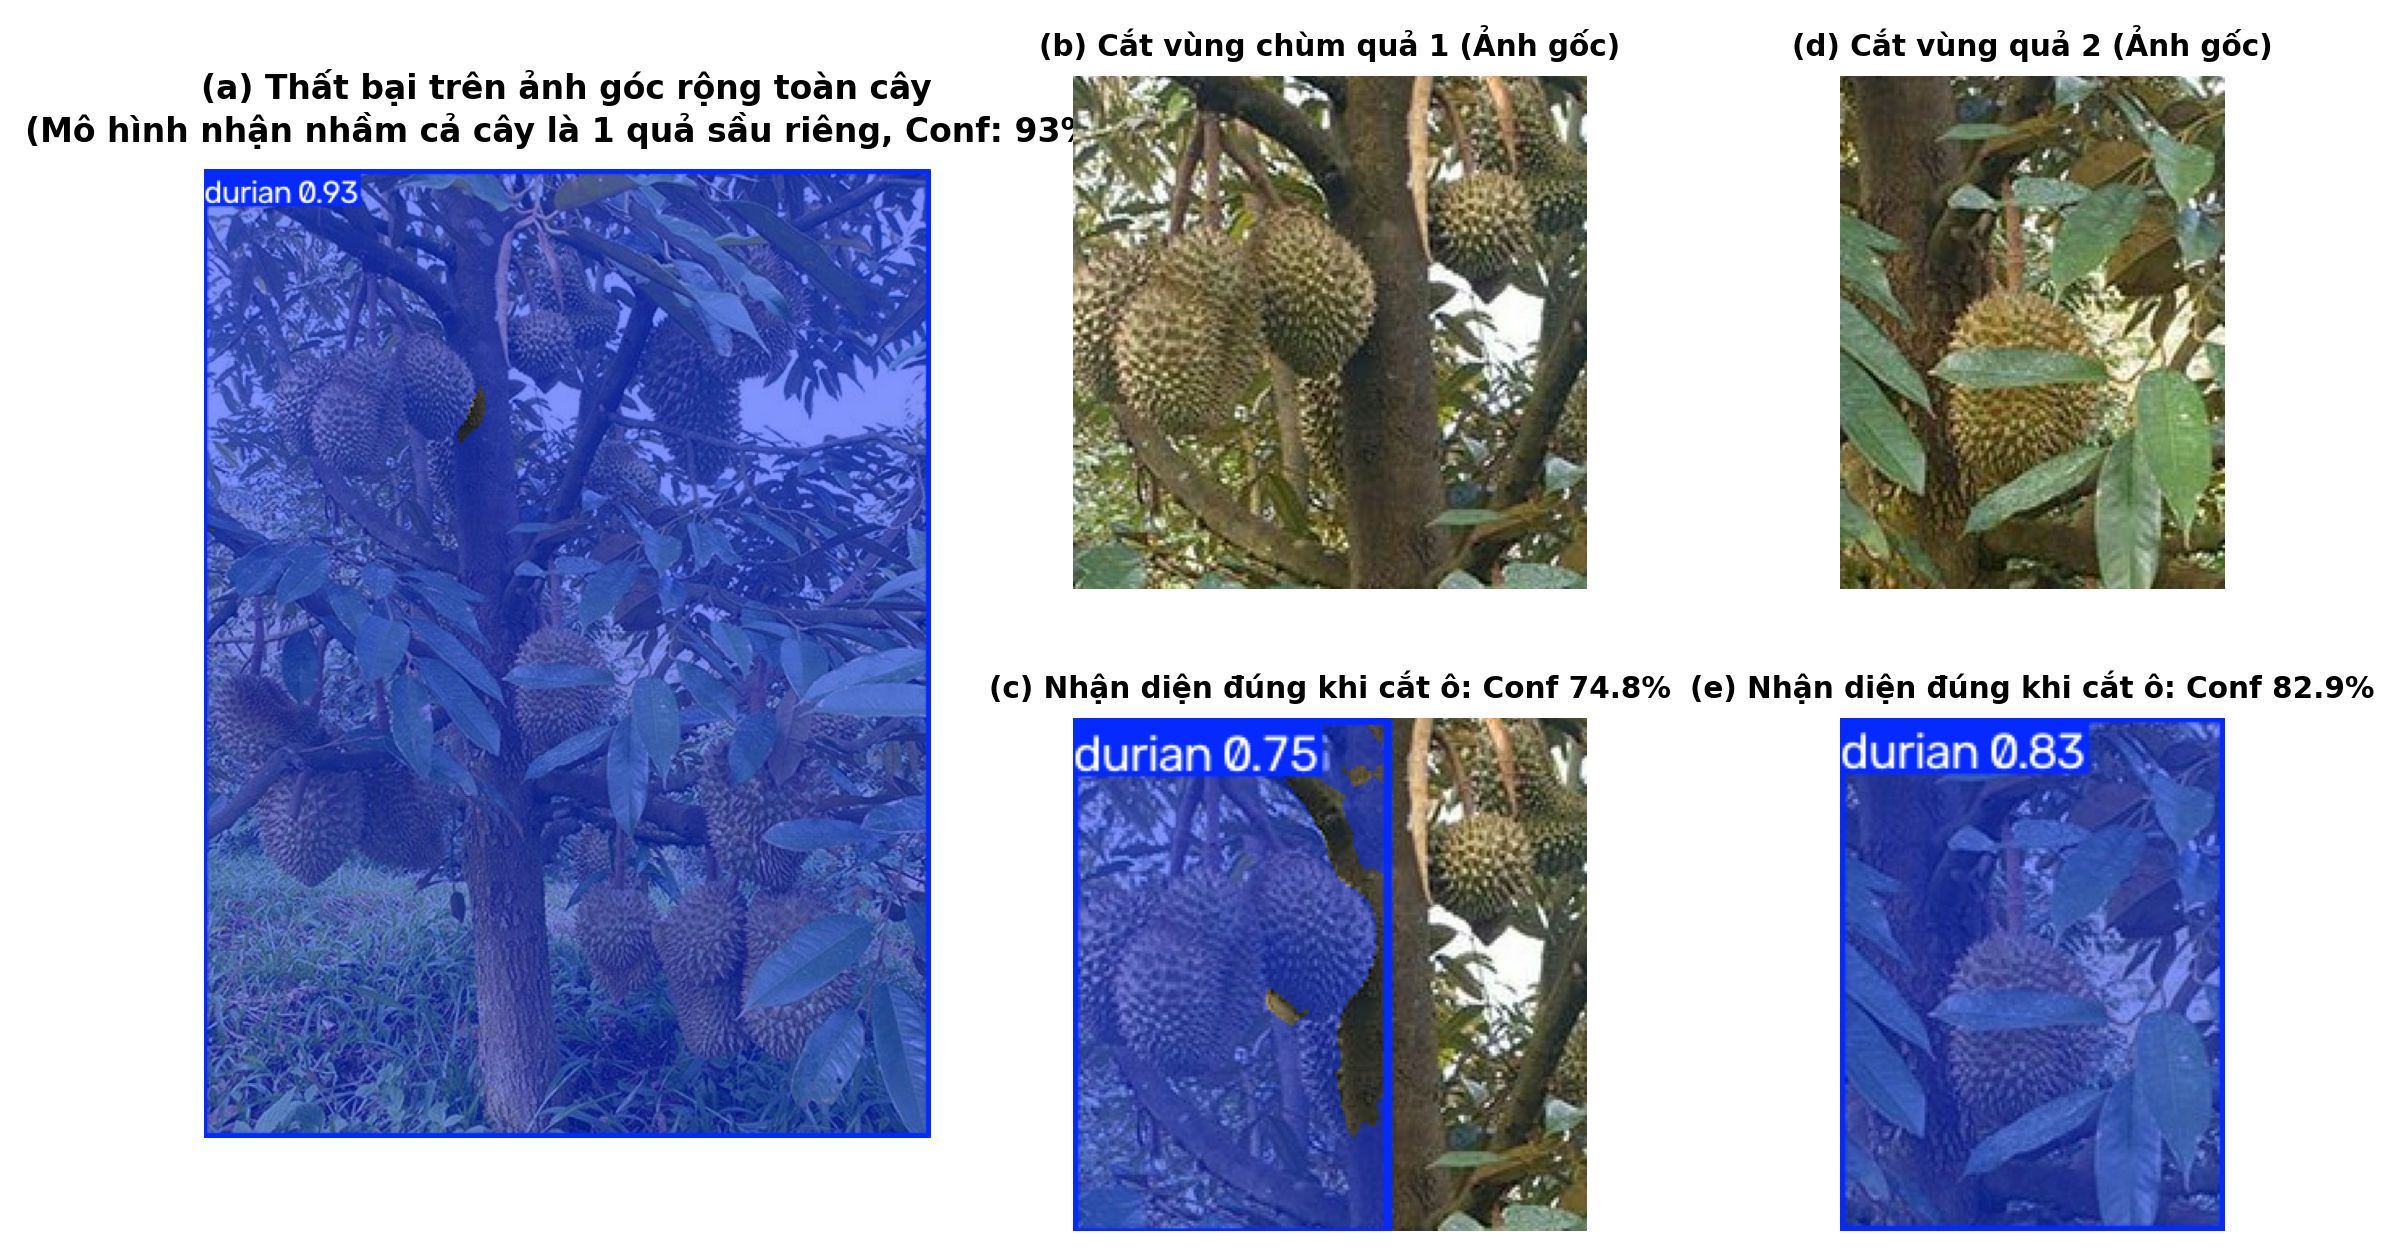
\includegraphics[width=0.98\textwidth]{scale_failure_analysis.png}
}{
    \framebox[0.98\textwidth]{\rule{0pt}{7.0cm} \textbf{FIGURE 3.1: SCALE COLLAPSE FAILURE ANALYSIS (scale\_failure\_analysis.png)}}
}
\caption{Empirical investigation of scale invariance failure and contextual overfitting on wide-angle canopy imagery (\texttt{sau-rieng2.jpg}). (a) The baseline model misclassifies the entire tree canopy as a single giant durian occupying $99.58\%$ of the image ($conf = 92.56\%$) due to extreme training scale bias. (b--c) Fruit cluster 1 patch: the model exhibits under-segmentation, clumping two adjacent fruits into a single entity ($conf = 74.8\%$) and completely missing the third fruit. (d--e) Fruit 2 patch: the model exhibits crop-filling bias ($conf = 82.9\%$), where the bounding box spans nearly $100\%$ of the patch and the mask bleeds severely onto the surrounding tree trunk and foliage.}
\label{fig:scale_failure}
\end{figure}

\paragraph{Root Cause Dataset Audit:}
A comprehensive audit of the 2,676 merged training annotations revealed the underlying causes:
\begin{enumerate}
    \item \textbf{Extreme Scale Bias in Aggregated Datasets:} Across all training images, the mean object count per image is exactly $1.00$, with target fruits occupying an average of $30.2\%$ of the image area (ranging up to $55\%$). Crucially, zero images depicted distant full-tree perspectives with small fruits occupying $1\text{--}2\%$ of the frame. The network was strongly conditioned to associate durian presence with dominant, frame-filling objects.
    \item \textbf{Contextual Overfitting from Sequential Video Frames:} A substantial portion of training data originated from consecutive video sequences (\texttt{frame\_0}, \texttt{frame\_10}, \texttt{frame\_20}...). The convolutional kernels memorized full-frame textured greenish-brown patterns. When presented with a full tree exhibiting similar overall coloration and rugged bark textures, the network's large receptive fields erroneously treated the entire canopy as a single fruit entity.
    \item \textbf{The Validation Metric Illusion:} The high validation Mask mAP@50 score ($0.9820$) was achieved because the validation set was randomly sampled from the same close-up repositories. This failure vividly illustrates how internal validation metrics can mask severe out-of-distribution (OOD) generalization deficits.
\end{enumerate}

\paragraph{Counter-Validation via Local Patch Slicing: Exposing Severe Contextual Overfitting:}
When local crops were extracted around fruit regions in \texttt{sau-rieng2.jpg} to restore the fruit area to proportions familiar from the training distribution ($20\%\text{--}30\%$ of the patch), the empirical results in Figure~\ref{fig:scale_failure}(b--e) uncovered critical underlying failure modes:
\begin{itemize}
    \item \textbf{Cluster 1 Crop (Figure~\ref{fig:scale_failure}c):} The cropped region contains three fruits (a clumped pair on the left and a separate fruit on the right). The model predicted a single bounding box merging the two clumped fruits into one single entity (\texttt{durian 0.75}), while completely omitting the third fruit (False Negative). This demonstrates an instance under-segmentation and clumping failure when fruits grow in natural dense clusters.
    \item \textbf{Fruit 2 Crop (Figure~\ref{fig:scale_failure}e):} The target fruit is suspended between leaves and the tree trunk. The model predicted a bounding box occupying almost $100\%$ of the entire cropped patch (\texttt{durian 0.83}), causing severe boundary bleeding where the segmentation mask spilled broadly across the tree trunk and surrounding leaves. This reveals a chronic ``crop-filling bias'': whenever a sub-patch is ingested, the network presumes a single object spans the whole window rather than resolving the true morphological boundaries of the fruit.
\end{itemize}
These empirical observations prove that: \textbf{The current model suffers from severe contextual overfitting to close-up single-fruit images}, and relying solely on post-hoc slicing algorithms (SAHI) without retraining on natural in-situ orchard data cannot resolve these fundamental boundary and instance-separation defects.

\noindent\textbf{Comprehensive Mitigation Roadmap for Sprint 4:}
\begin{enumerate}
    \item \textbf{In-situ Orchard Dataset Collection:} Collect 300--500 high-resolution full-canopy and mid-range images directly in natural durian orchards across varying illumination conditions, camera distances ($0.5\text{--}5.0\,\text{m}$), and heavy cluster occlusions.
    \item \textbf{Automated Polygon Labeling via Foundation Models (Grounded-SAM):} To circumvent the bottleneck of manual polygon annotation (which requires hundreds of manual vertex clicking hours), we implement a zero-shot semi-automated annotation pipeline: Combining \textbf{Grounding DINO} \cite{liu2023grounding} with \textbf{Segment Anything (SAM / SAM 2)} \cite{kirillov2023segment}. High-level text prompts (\texttt{``durian fruit''}) direct Grounding DINO to propose rough bounding boxes, which are instantly ingested by SAM as prompt boxes to extract sub-pixel precision polygon contours. Human annotators act exclusively as rapid quality assurance auditors (Human-in-the-loop verification), boosting annotation throughput by $20\text{--}30\times$.
    \item \textbf{Scale-Jittered Copy-Paste Augmentation and SAHI Fine-Tuning:} Synthesize diverse fruit scales by randomly blending segmented fruits at small scale ratios ($0.05\text{--}0.25$) onto complex orchard canopy backgrounds, followed by fine-tuning YOLOv8n-seg alongside the SAHI inference framework \cite{akyon2022sahi}.
\end{enumerate}

\subsubsection{Physical and Hardware Constraints}
\begin{enumerate}
    \item \textbf{Solar Infrared Radiation Washout on RealSense D453i:}
    The Intel RealSense D453i active stereoscopic depth sensor relies on an infrared pattern projector. Under intense tropical sunlight, ambient solar infrared radiation ($\approx 850\,\text{nm}$ and $940\,\text{nm}$) washes out the projected pattern, producing zero-depth voids on sunlit fruit surfaces. In Sprint 4, we will deploy optical bandpass filters and implement a mask-bounded depth spatial inpainting algorithm strictly constrained within $M(u, v)$.
    
    \item \textbf{UGV Chassis Vibration and Terrain Dynamics:}
    Traversing terraced orchard terrain induces mechanical shock and vibrations. These dynamics cause motion blur on color frames and introduce temporal misalignments between RGB and depth frames of the RealSense D453i as well as LiDAR C1M1 scan lines. In our physical integration, rubber dampening mounts and the built-in 6-DOF IMU of the RealSense D453i will be utilized for real-time kinematic motion compensation.
    
    \item \textbf{Software Licensing Constraints (AGPL-3.0 vs. Commercial Deployment):}
    Ultralytics YOLOv8 is released under the GNU Affero General Public License v3.0 (AGPL-3.0), which requires commercial systems interacting with the codebase to publish their proprietary source code. The project decouples model training from runtime inference: trained weights are exported to standalone ONNX formats and executed via an independent C++ ROS 2 node using ONNX Runtime / NCNN on the Raspberry Pi 5, isolating the commercial robotics software stack from AGPL runtime dependencies.
\end{enumerate}
% ==============================================================================
% SECTION 4: NEXT WORK
% ==============================================================================
\section{Next work}

Table~\ref{tab:plan} details our roadmap and deliverables for Sprint 4 (covering the period 26 Oct -- 08 Nov 2026, corresponding to Progress Report 4).

\begin{table}[htbp]
\centering
\small
\caption{Planned tasks and milestone deliverables for 26 Oct -- 08 Nov 2026 (Report 4 sprint).}
\label{tab:plan}
\begin{tabularx}{\textwidth}{c p{7.0cm} X}
\toprule
\textbf{Task} & \textbf{Task Description} & \textbf{Target Deliverable / Output} \\
\midrule
\textbf{1} & Package the baseline YOLOv8n-seg model and the MF-3DLoc algorithm into a standalone ROS 2 Jazzy perception node for Raspberry Pi 5 (16\,GB). & Clean ROS 2 node subscribing to RealSense D453i topics, integrating SAHI multi-scale slicing for wide-angle canopy views, and optimized via ONNX Runtime / NCNN on ARM NEON. \\
\addlinespace
\textbf{2} & Implement dynamic TF2 spatial coordinate transformations from the RealSense D453i optical frame to the turret base link. & Published target coordinate topic \texttt{/turret/target\_3d\_goal} containing stamped spatial vectors $(X_T, Y_T, Z_T)$ with confidence metadata. \\
\addlinespace
\textbf{3} & Validate closed-loop tracking and turret aim accuracy in a high-fidelity Gazebo orchard simulation environment integrated with LiDAR C1M1 data. & Gazebo simulation demonstration under simulated UGV vibration and sloped terrain, measuring dynamic targeting precision. \\
\bottomrule
\end{tabularx}
\end{table}

% ==============================================================================
% SECTION 5: MAPPING TO COURSE LEARNING OUTCOMES
% ==============================================================================
\section{Mapping of the work to course learning outcomes}

Table~\ref{tab:clo_mapping} provides the mapping connecting the experimental and engineering work completed in this sprint (12 Oct -- 25 Oct 2026) directly to the CO3133 course learning outcomes.

\begin{table}[htbp]
\centering
\small
\caption{Detailed mapping of project deliverables to CO3133 Course Learning Outcomes.}
\label{tab:clo_mapping}
\begin{tabularx}{\textwidth}{>{\raggedright\arraybackslash}p{6.5cm} c X c}
\toprule
\textbf{Completed Technical Work} & \textbf{C\DJ R Mapping} & \textbf{Course Syllabus Description} & \textbf{Status} \\
\midrule
Execution of 5-scenario ablation benchmark on RTX 3060 (Table~2.1), multi-task loss analysis (Figure~2.1), mosaic deactivation dynamics, confusion matrix error breakdown, and Wilson 95\% confidence interval. & \textbf{C\DJ R 8 (L.O.5.1)} & Apply quantitative metrics, ablation protocols, and error decomposition to evaluate deep learning performance on domain data. & \textbf{Done} \\
\addlinespace
Architectural trade-off analysis (YOLOv8n-seg vs. YOLOv8s-seg), resolution and batch size evaluation, Raspberry Pi 5 (16\,GB) CPU/RAM resource budget planning, RealSense D453i, and LiDAR C1M1 (Section~3). & \textbf{C\DJ R 9 (L.O.5.2)} & Formulate and justify technical model selection under embedded edge constraints (latency, throughput, memory, power). & \textbf{Done} \\
\addlinespace
Configuration and execution of GPU-accelerated deep learning pipelines using PyTorch 2.3.0 and Ultralytics 8.2 on an NVIDIA RTX 3060 workstation (Section~1.3, Section~2). & \textbf{C\DJ R 4 (L.O.4.1)} & Implement and fine-tune deep learning models using modern software toolkits on GPU computing infrastructure. & \textbf{Done} \\
\addlinespace
Multi-source dataset aggregation (5 Roboflow repositories), polygon standardization and sanitization via \texttt{merge\_datasets.py}, and online GPU augmentation monitoring (Section~2.1). & \textbf{C\DJ R 5 (L.O.4.2)} & Design data preprocessing, sanitization, and augmentation strategies to ensure data integrity and prevent overfitting. & \textbf{Done} \\
\bottomrule
\end{tabularx}
\end{table}

\newpage
% REFERENCES
% ==============================================================================
\begin{thebibliography}{10}

\bibitem{ultralytics2023}
G.~Jocher, A.~Chaurasia, and J.~Kwon, ``Ultralytics YOLOv8,'' 2023. [Online]. Available: \url{https://github.com/ultralytics/ultralytics}

\bibitem{zheng2020ciou}
Z.~Zheng, P.~Wang, W.~Liu, J.~Li, R.~Ye, and D.~Ren, ``Distance-IoU loss: Faster and better learning for bounding box regression,'' in \textit{Proceedings of the AAAI Conference on Artificial Intelligence}, vol.~34, no.~07, 2020, pp. 12\,993--13\,000.

\bibitem{li2020generalized}
X.~Li, C.~Lv, W.~Wang, G.~Li, L.~Yang, and J.~Yang, ``Generalized focal loss: Learning qualified and distributed bounding boxes for dense object detection,'' in \textit{Advances in Neural Information Processing Systems (NeurIPS)}, vol.~33, 2020, pp. 21\,002--21\,012.

\bibitem{macenski2020marathon}
S.~Macenski, F.~Mart{\'\i}n, R.~White, and J.~Gin{\'e}s Clavero, ``The Marathon 2: A navigation system,'' in \textit{IEEE/RSJ International Conference on Intelligent Robots and Systems (IROS)}, 2020, pp. 2718--2725.

\bibitem{he2017maskrcnn}
K.~He, G.~Gkioxari, P.~Doll{\'a}r, and R.~Girshick, ``Mask R-CNN,'' in \textit{IEEE/CVF International Conference on Computer Vision (ICCV)}, 2017, pp. 2961--2969.

\bibitem{bolya2019yolact}
D.~Bolya, C.~Zhou, F.~Xiao, and Y.~J.~Lee, ``YOLACT: Real-time instance segmentation,'' in \textit{IEEE/CVF International Conference on Computer Vision (ICCV)}, 2019, pp. 9157--9166.

\bibitem{wilson1927probable}
E.~B.~Wilson, ``Probable inference, the law of succession, and statistical inference,'' \textit{Journal of the American Statistical Association}, vol.~22, no.~158, pp. 209--212, 1927.

\bibitem{fu2020rgbd}
L.~Fu, F.~Gao, J.~Wu, R.~Li, M.~Karkee, and Q.~Zhang, ``Application of consumer RGB-D cameras for fruit detection and localization in field: A critical review,'' \textit{Computers and Electronics in Agriculture}, vol.~177, p. 105687, 2020. [Online]. DOI: \url{https://doi.org/10.1016/j.compag.2020.105687}

\bibitem{lin2021fruit}
G.~Lin, Y.~Tang, X.~Zou, and C.~Wang, ``Three-dimensional reconstruction of fruits and branches using instance segmentation and geometry analysis,'' \textit{Computers and Electronics in Agriculture}, vol.~184, p. 106107, 2021. [Online]. DOI: \url{https://doi.org/10.1016/j.compag.2021.106107}

\bibitem{kang2020dasnet}
H.~Kang and C.~Chen, ``Fruit detection, segmentation and 3D visualisation of environments in apple orchards,'' \textit{Computers and Electronics in Agriculture}, vol.~171, p. 105302, 2020. [Online]. DOI: \url{https://doi.org/10.1016/j.compag.2020.105302}

\bibitem{akyon2022sahi}
F.~C.~Akyon, S.~O.~Altinuc, and A.~Temizel, ``Slicing Aided Hyper Inference and fine-tuning for small object detection,'' in \textit{IEEE International Conference on Image Processing (ICIP)}, 2022, pp. 966--970. [Online]. DOI: \url{https://doi.org/10.1109/ICIP46576.2022.9897990}
\bibitem{kirillov2023segment}
A.~Kirillov, E.~Mintun, N.~Ravi, H.~Mao, C.~Rolland, L.~Gustafson, T.~Xiao, S.~Whitehead, A.~C.~Berg, W.-Y.~Lo, P.~Doll{\'a}r, and R.~Girshick, `Segment anything,'' in \textit{Proceedings of the IEEE/CVF International Conference on Computer Vision (ICCV)}, 2023, pp. 4015--4026. [Online]. DOI: \url{https://doi.org/10.1109/ICCV51070.2023.00371}

\bibitem{liu2023grounding}
S.~Liu, Z.~Zeng, T.~Ren, F.~Li, H.~Zhang, J.~Yang, C.~Li, J.~Yang, H.~Su, J.~Zhu, and L.~Zhang, `Grounding DINO: Marrying DINO with grounded pre-training for open-set object detection,'' in \textit{Proceedings of the European Conference on Computer Vision (ECCV)}, 2024. [Online]. arXiv:2303.05499.

\end{thebibliography}

\end{document}
\subsubsection{Cluster Occlusion Case Study on \texttt{sau-rieng3.jpg}: Missed Detections in Overlapping Fruits}
To evaluate model behavior when encountering dense fruit clusters in natural orchards, inference was executed on \texttt{sau-rieng3.jpg}. This real orchard scene contains a cluster of \textbf{3 durians growing in close proximity and heavily overlapping each other}:
\begin{itemize}
    \item \textbf{Empirical Observation:} The model successfully detects \textbf{only 1 dominant foreground durian} with $91.79\%$ confidence (BBox $[164.1, 118.1, 702.3, 395.7]$ covering $31.13\%$ of the frame), while the \textbf{2 occluded durians behind it are completely missed (False Negatives)}!
    \item \textbf{Root Cause Analysis:}
    \begin{enumerate}
        \item \textit{Single-Fruit Dataset Bias:} The Roboflow training set (1,053 images) contains predominantly isolated fruits (mean $1.2$ fruits/image). The convolutional backbone was never exposed to dense clusters with heavy occlusion.
        \item \textit{Spike Texture Homogenization:} All fruits share identical greenish-brown spiky textures. At overlapping contact boundaries, the absence of sharp contrast borders causes convolutional feature maps to assimilate the cluster into the dominant foreground instance.
        \item \textit{Non-Maximum Suppression (NMS) Elimination:} Candidate proposals for the background fruits exhibit high spatial IoU overlap with the foreground fruit's bounding box, resulting in their suppression by standard NMS ($\text{IoU} = 0.7$).
    \end{enumerate}
    \item \textbf{Mitigation Strategy for Sprint 4:} Incorporating synthetic Copy-Paste overlap augmentation ($30\text{--}70\%$ occlusion), adopting \textbf{Soft-NMS} or \textbf{Mask-guided NMS} (using mask IoU rather than bounding box IoU to avoid spurious suppression), and deploying \textbf{Active Multi-view Vision} on the robot manipulator ($\pm 25^\circ$ viewpoint shifting to segment fruits in 3D depth point clouds).
\end{itemize}


